\documentclass[a4paper,12pt]{book}
%\usepackage[indonesian]{babel}
\usepackage{longtable}
\usepackage[utf8]{inputenc}
\usepackage{xcolor}
\usepackage{listings}
\usepackage{amsmath}
\usepackage{graphicx}
\usepackage{hyperref}
\usepackage[font=small,labelfont=bf]{caption}
\usepackage{float}
\usepackage{verbatim}

%\usepackage{geometry}
%\geometry{
%	a4paper,
%% 	total={170mm,257mm},
%	left=40mm,
%	top=30mm,
%	right=30mm,
%	bottom=30mm
%}
\hypersetup{
colorlinks = true,
urlcolor = blue,
linkcolor = blue,
citecolor = {blue!50!black}
}
\usepackage[a4paper,vmargin=3cm,rmargin=3cm,lmargin=4cm]{geometry}
\usepackage{xcolor}
\makeatletter
    \def\cleardoublepage{\clearpage%
        \if@twoside
            \ifodd\c@page\else
                \vspace*{\fill}
                \hfill
                \begin{center}
                This page is intentionaly left blank.
                \end{center}
                \vspace{\fill}
                \thispagestyle{empty}
                \newpage
                \if@twocolumn\hbox{}\newpage\fi
            \fi
        \fi
    }
\makeatother
%Code listing style pak akok
\definecolor{codegreen}{rgb}{0,0.6,0}
\definecolor{codegray}{rgb}{0.5,0.5,0.5}
\definecolor{codepurple}{rgb}{0.58,0,0.82}
\definecolor{backcolour}{rgb}{0.95,0.95,0.92}

\lstdefinestyle{mystyle}{
	backgroundcolor=\color{backcolour}, commentstyle=\color{codegreen},
	keywordstyle=\color{magenta},
	numberstyle=\small\color{codegray},
	stringstyle=\color{codepurple},
	basicstyle=\ttfamily\footnotesize,
	breakatwhitespace=false,         
	breaklines=true,                 
	captionpos=t,                    
	keepspaces=true,                 
	numbers=left,                    
	numbersep=5pt,                  
	showspaces=false,                
	showstringspaces=false,
	showtabs=false,           
	frame = single,
	tabsize=2
}
\lstset{style=mystyle}


\setcounter{tocdepth}{6}
\setcounter{secnumdepth}{6}


\begin{document}
\title{Basic Programming Lab Module}
\date{}
\author{}
\frontmatter
\maketitle
\tableofcontents

\mainmatter
\chapter{Structure of C Programming Language}
\section{Goals}
\begin{itemize}
%    \setlength\itemsep{0.5em}
	\item Students are able to create projects on an IDE
	\item Students can demonstrate his/her knowledge of the structure of a C program
	\item Students can demonstrate his/her knowledge of C data types
	\item Students can demonstrate his/her knowledge of C operators
    \item Students are able to use function to read inputs from keyboard
    \item Students are able to use function to print texts on screen
\end{itemize}
\section{Creating new projects on an IDE Code::Blocks}
\subsection{Steps to create a new project}
\begin{enumerate}
\item Go to File $>$ New $>$ Project 
	\begin{figure}[H]
		\centering
		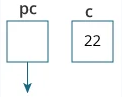
\includegraphics[width=0.7\linewidth]{StrukturProgramC/screenshot002}
		\caption{}
		\label{fig:screenshot002}
	\end{figure}
\item Click Console Application
\begin{figure}[H]
	\centering
	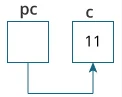
\includegraphics[width=0.7\linewidth]{StrukturProgramC/screenshot004}
	\caption{}
	\label{fig:screenshot004}
\end{figure}
\item Choose C as programming language
\begin{figure}[H]
	\centering
	\includegraphics[width=0.7\linewidth]{StrukturProgramC/screenshot005}
	\caption{}
	\label{fig:screenshot005}
\end{figure}
\item Give a name to the project
\begin{figure}[H]
	\centering
	\includegraphics[width=0.7\linewidth]{StrukturProgramC/screenshot006}
	\caption{}
	\label{fig:screenshot006}
\end{figure}
\item  Choose the compiler (gcc), set the saving directory, and click finish.
\begin{figure}[H]
	\centering
	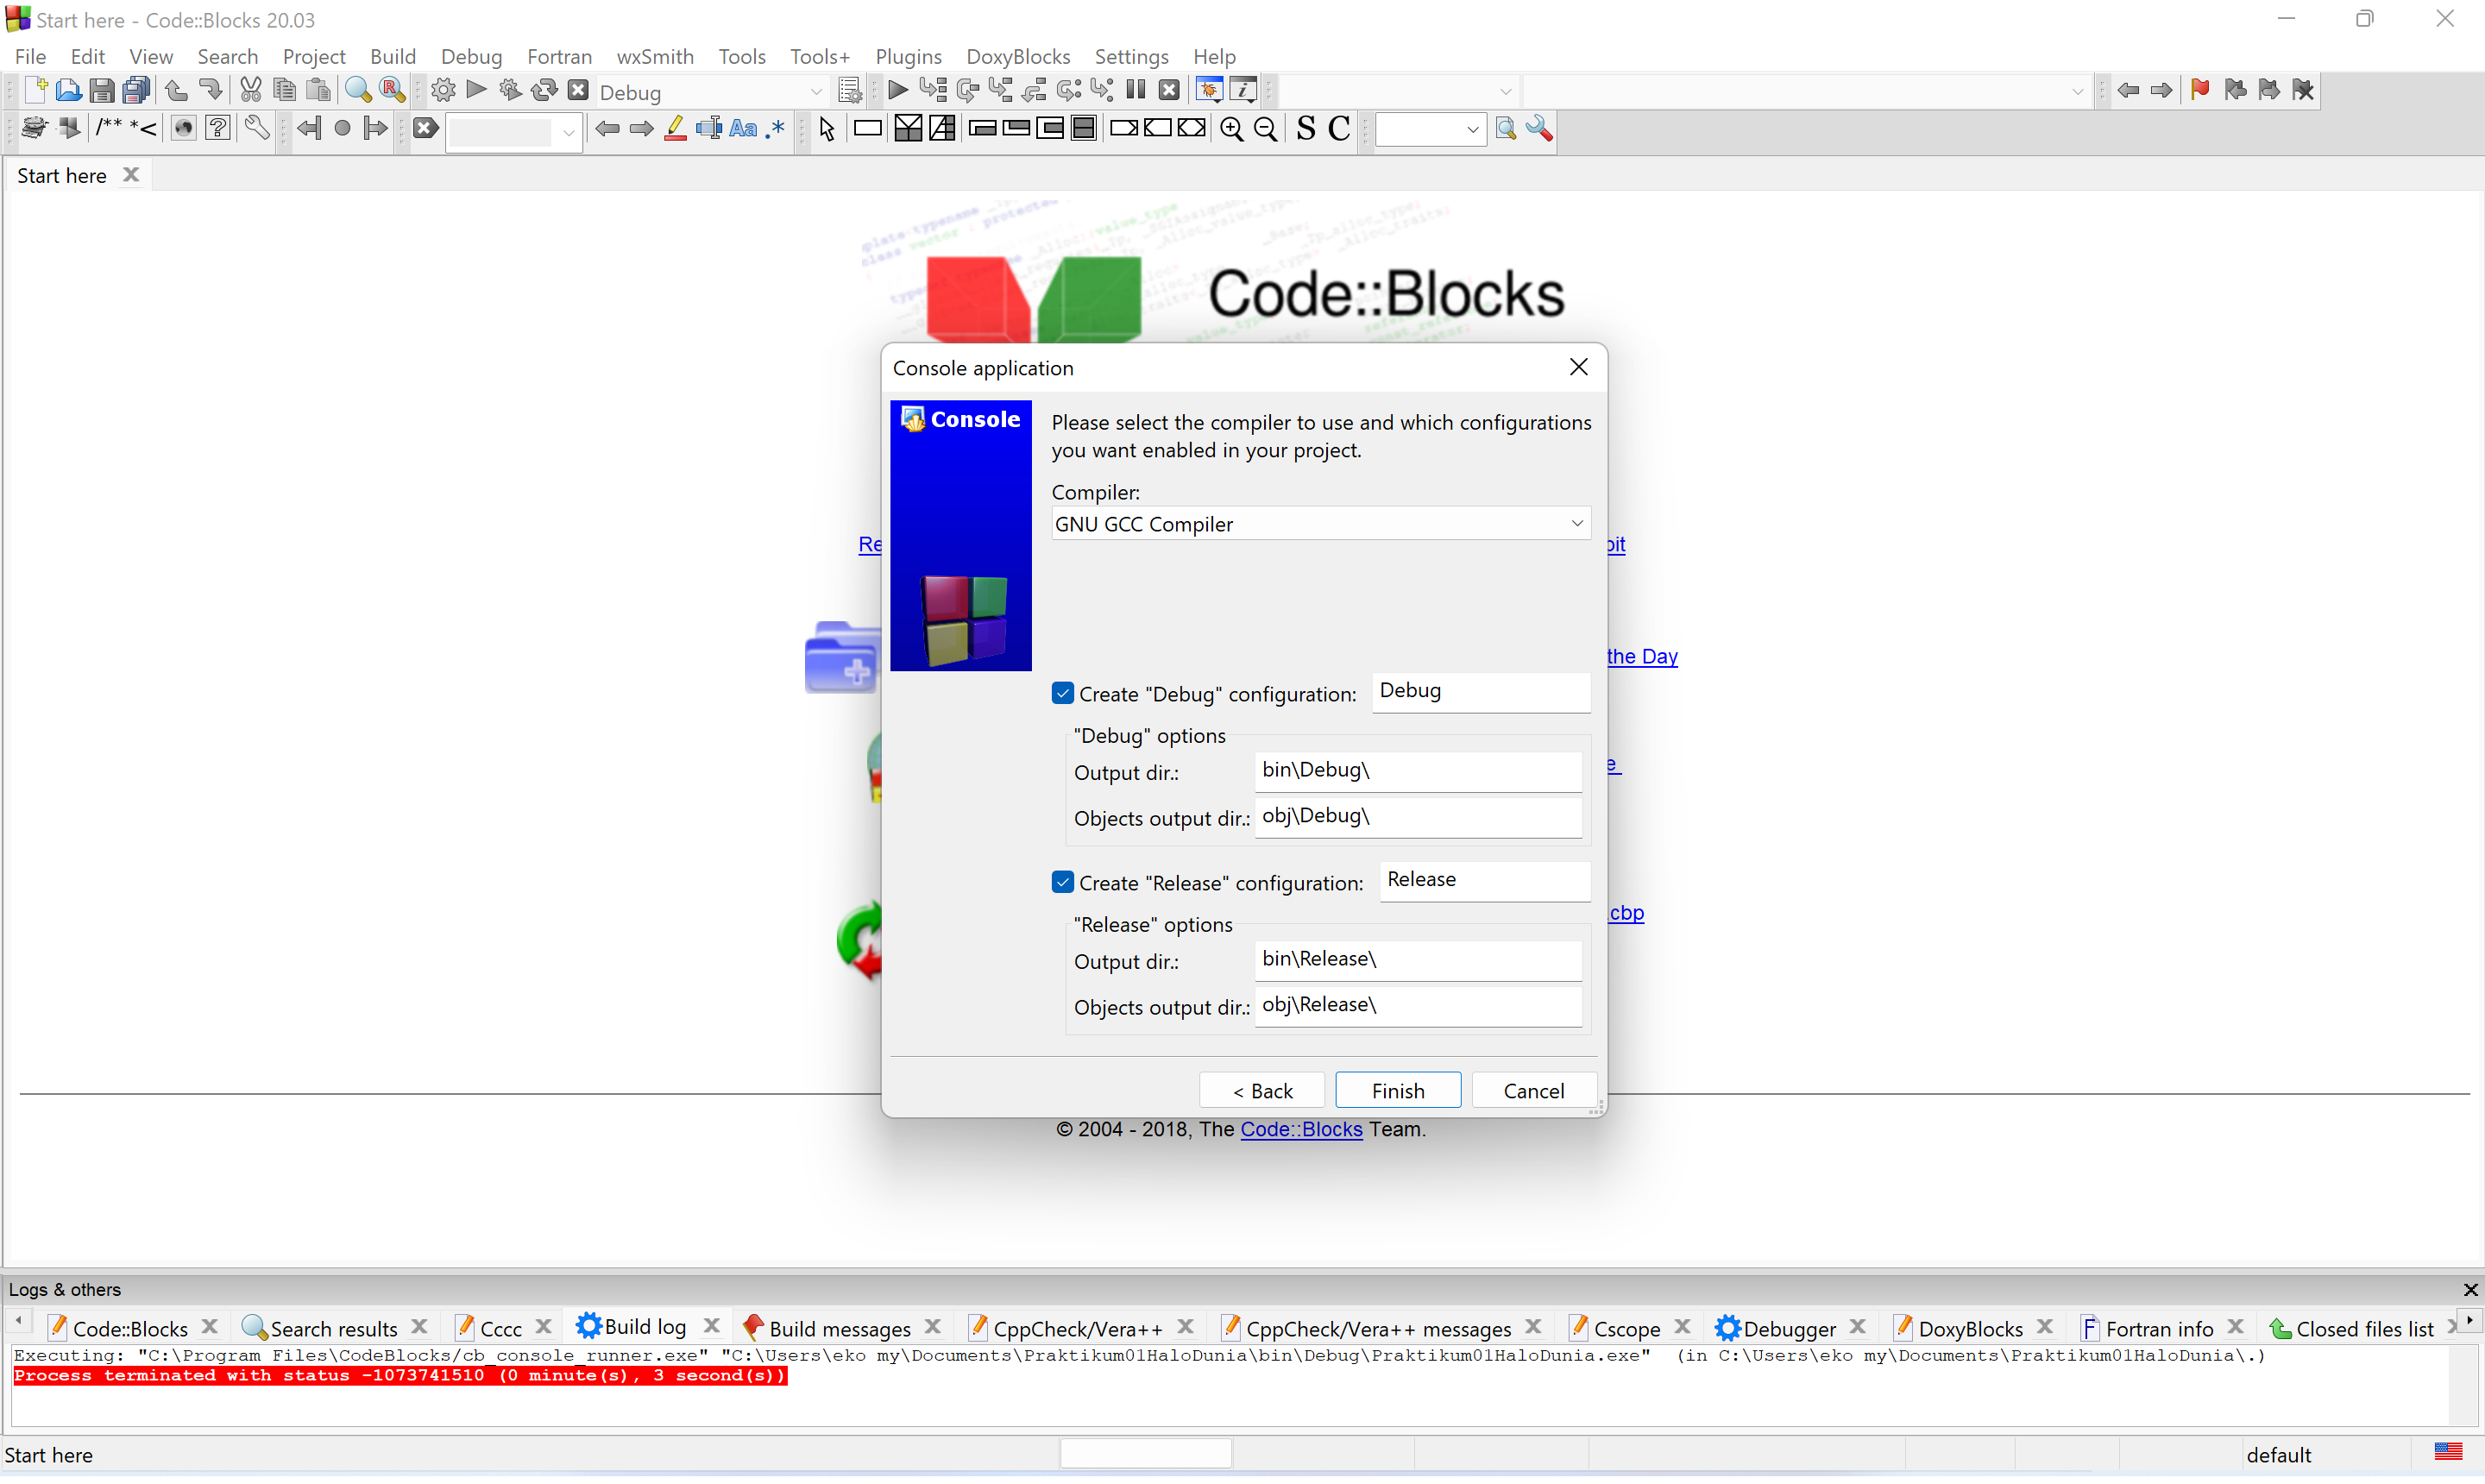
\includegraphics[width=0.7\linewidth]{StrukturProgramC/screenshot007}
	\caption{}
	\label{fig:screenshot007}
\end{figure}
\item Type the code in figure \ref{fig:screenshot008} to the Code::Blocks text editor
\begin{figure}[H]
	\centering
	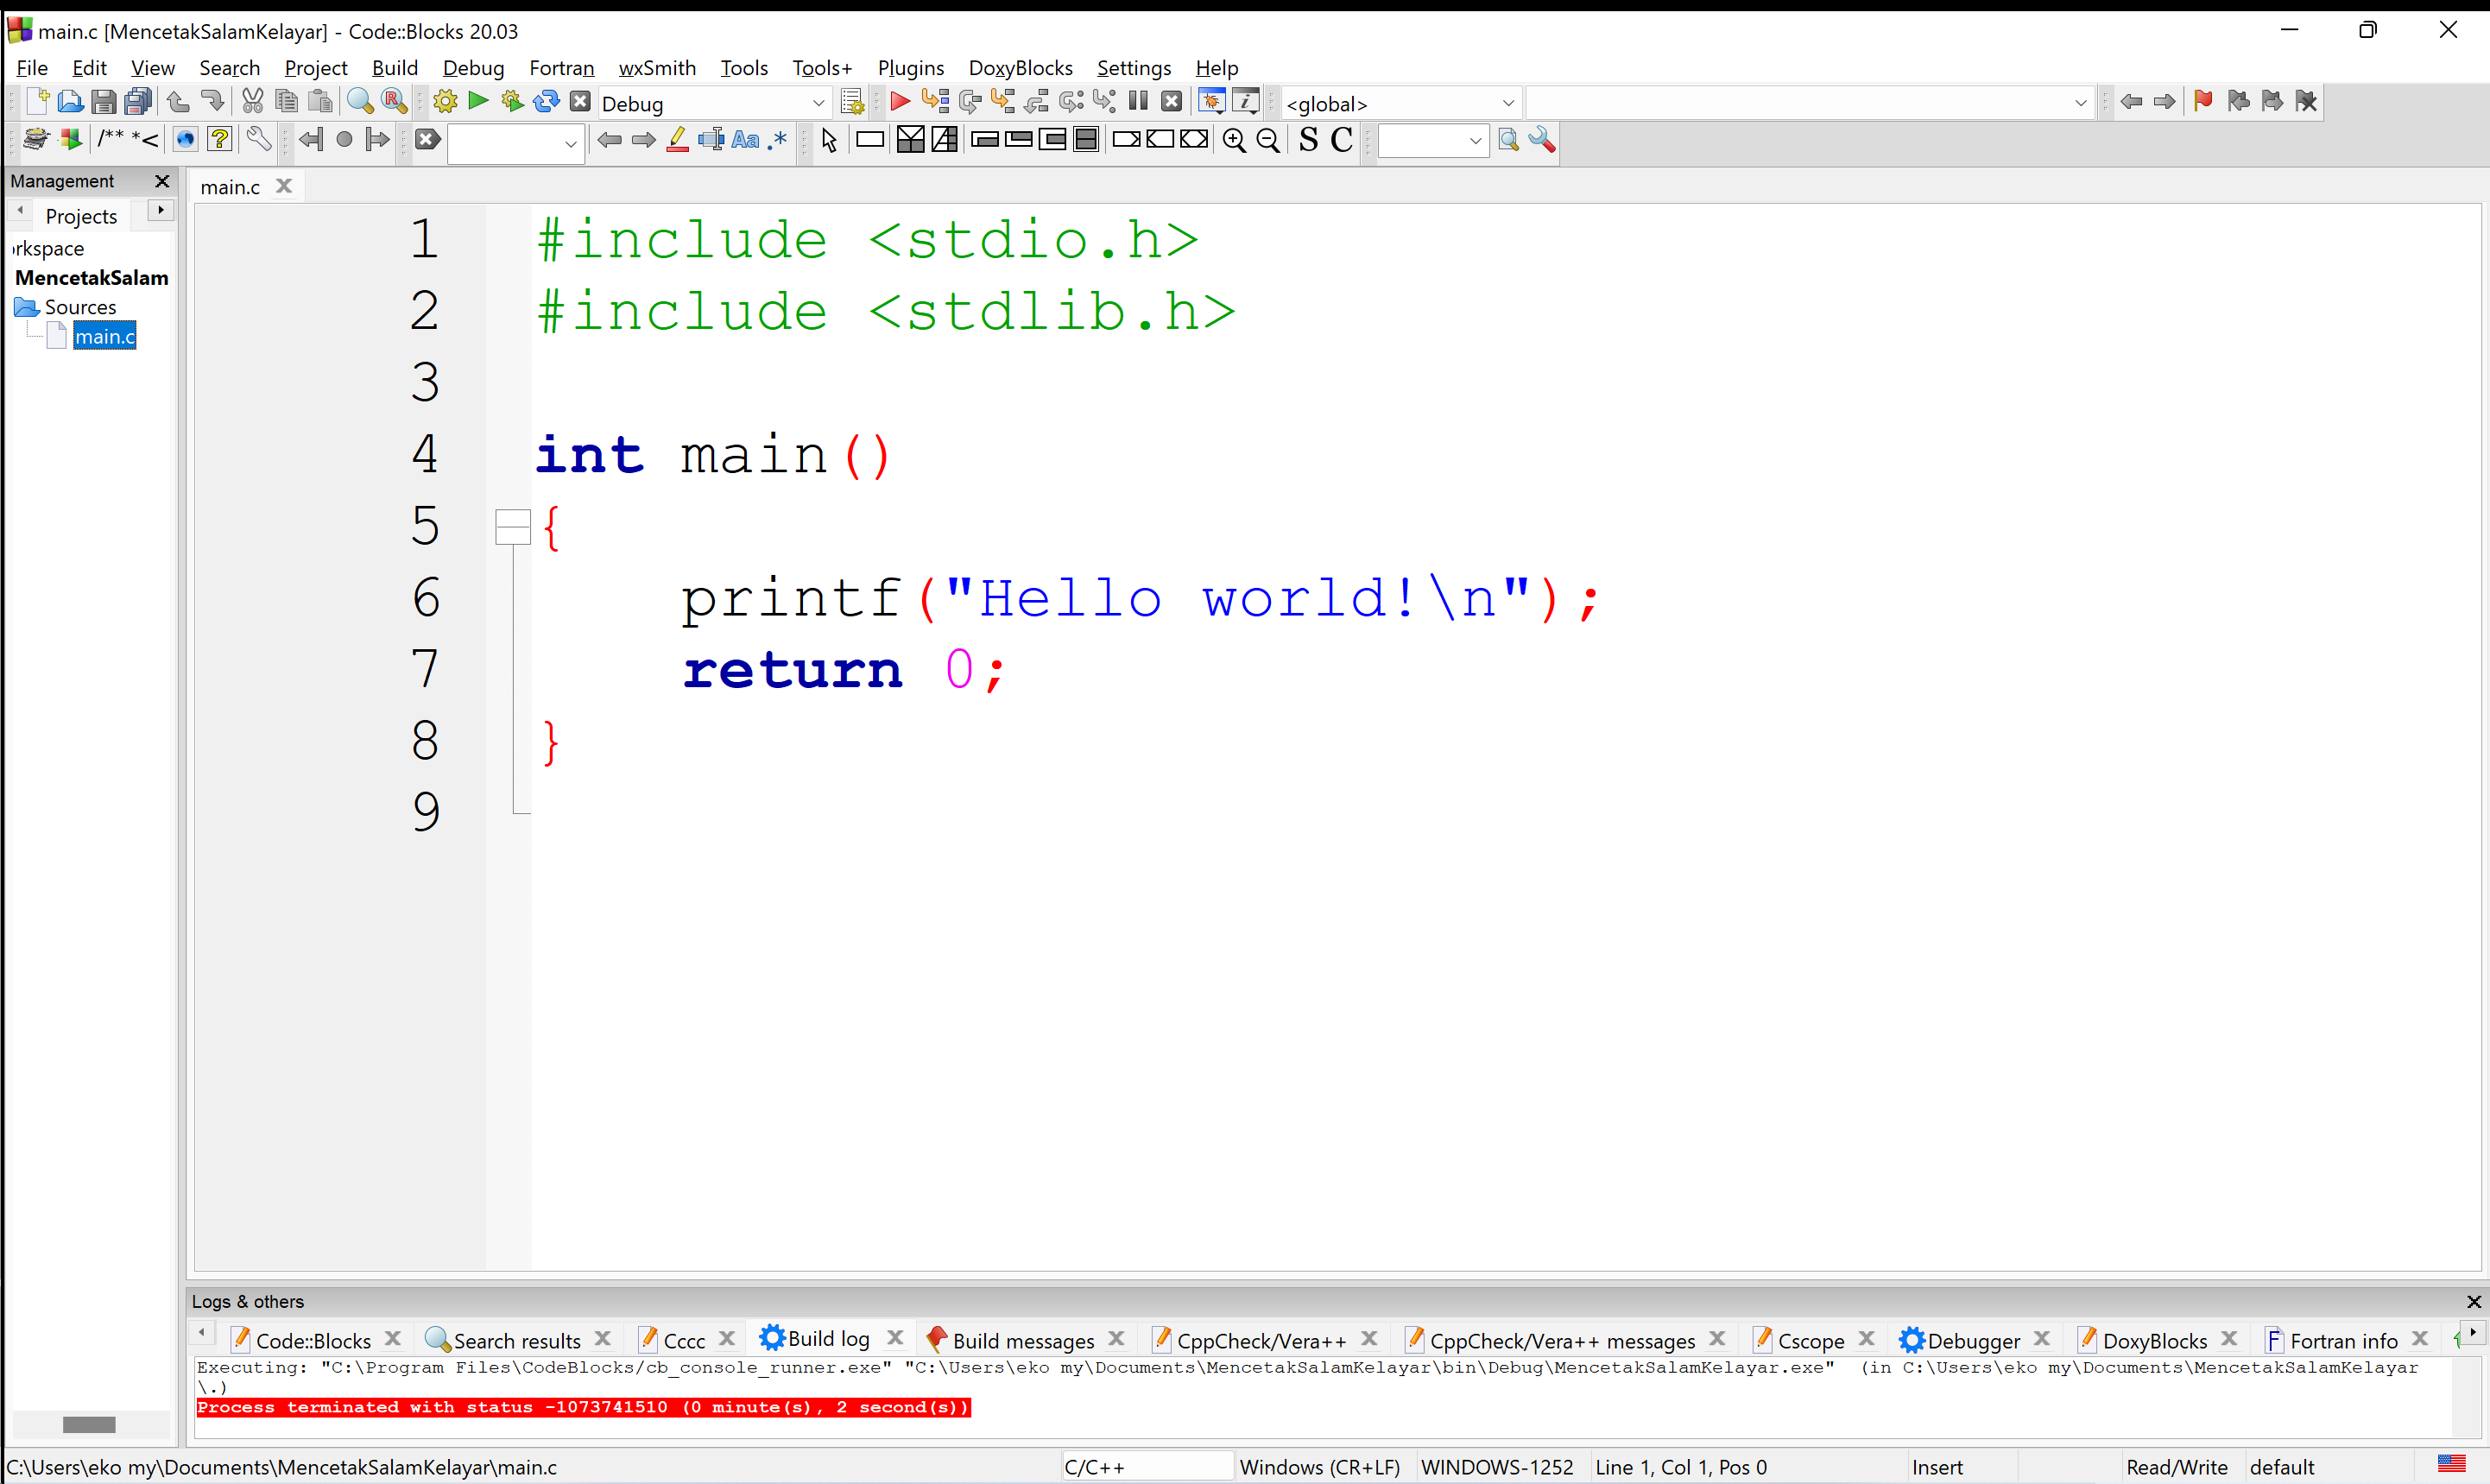
\includegraphics[width=0.7\linewidth]{StrukturProgramC/screenshot008}
	\caption{}
	\label{fig:screenshot008}
\end{figure}
\item click Build$->$Build and Run or press F9
\begin{figure}[H]
	\centering
	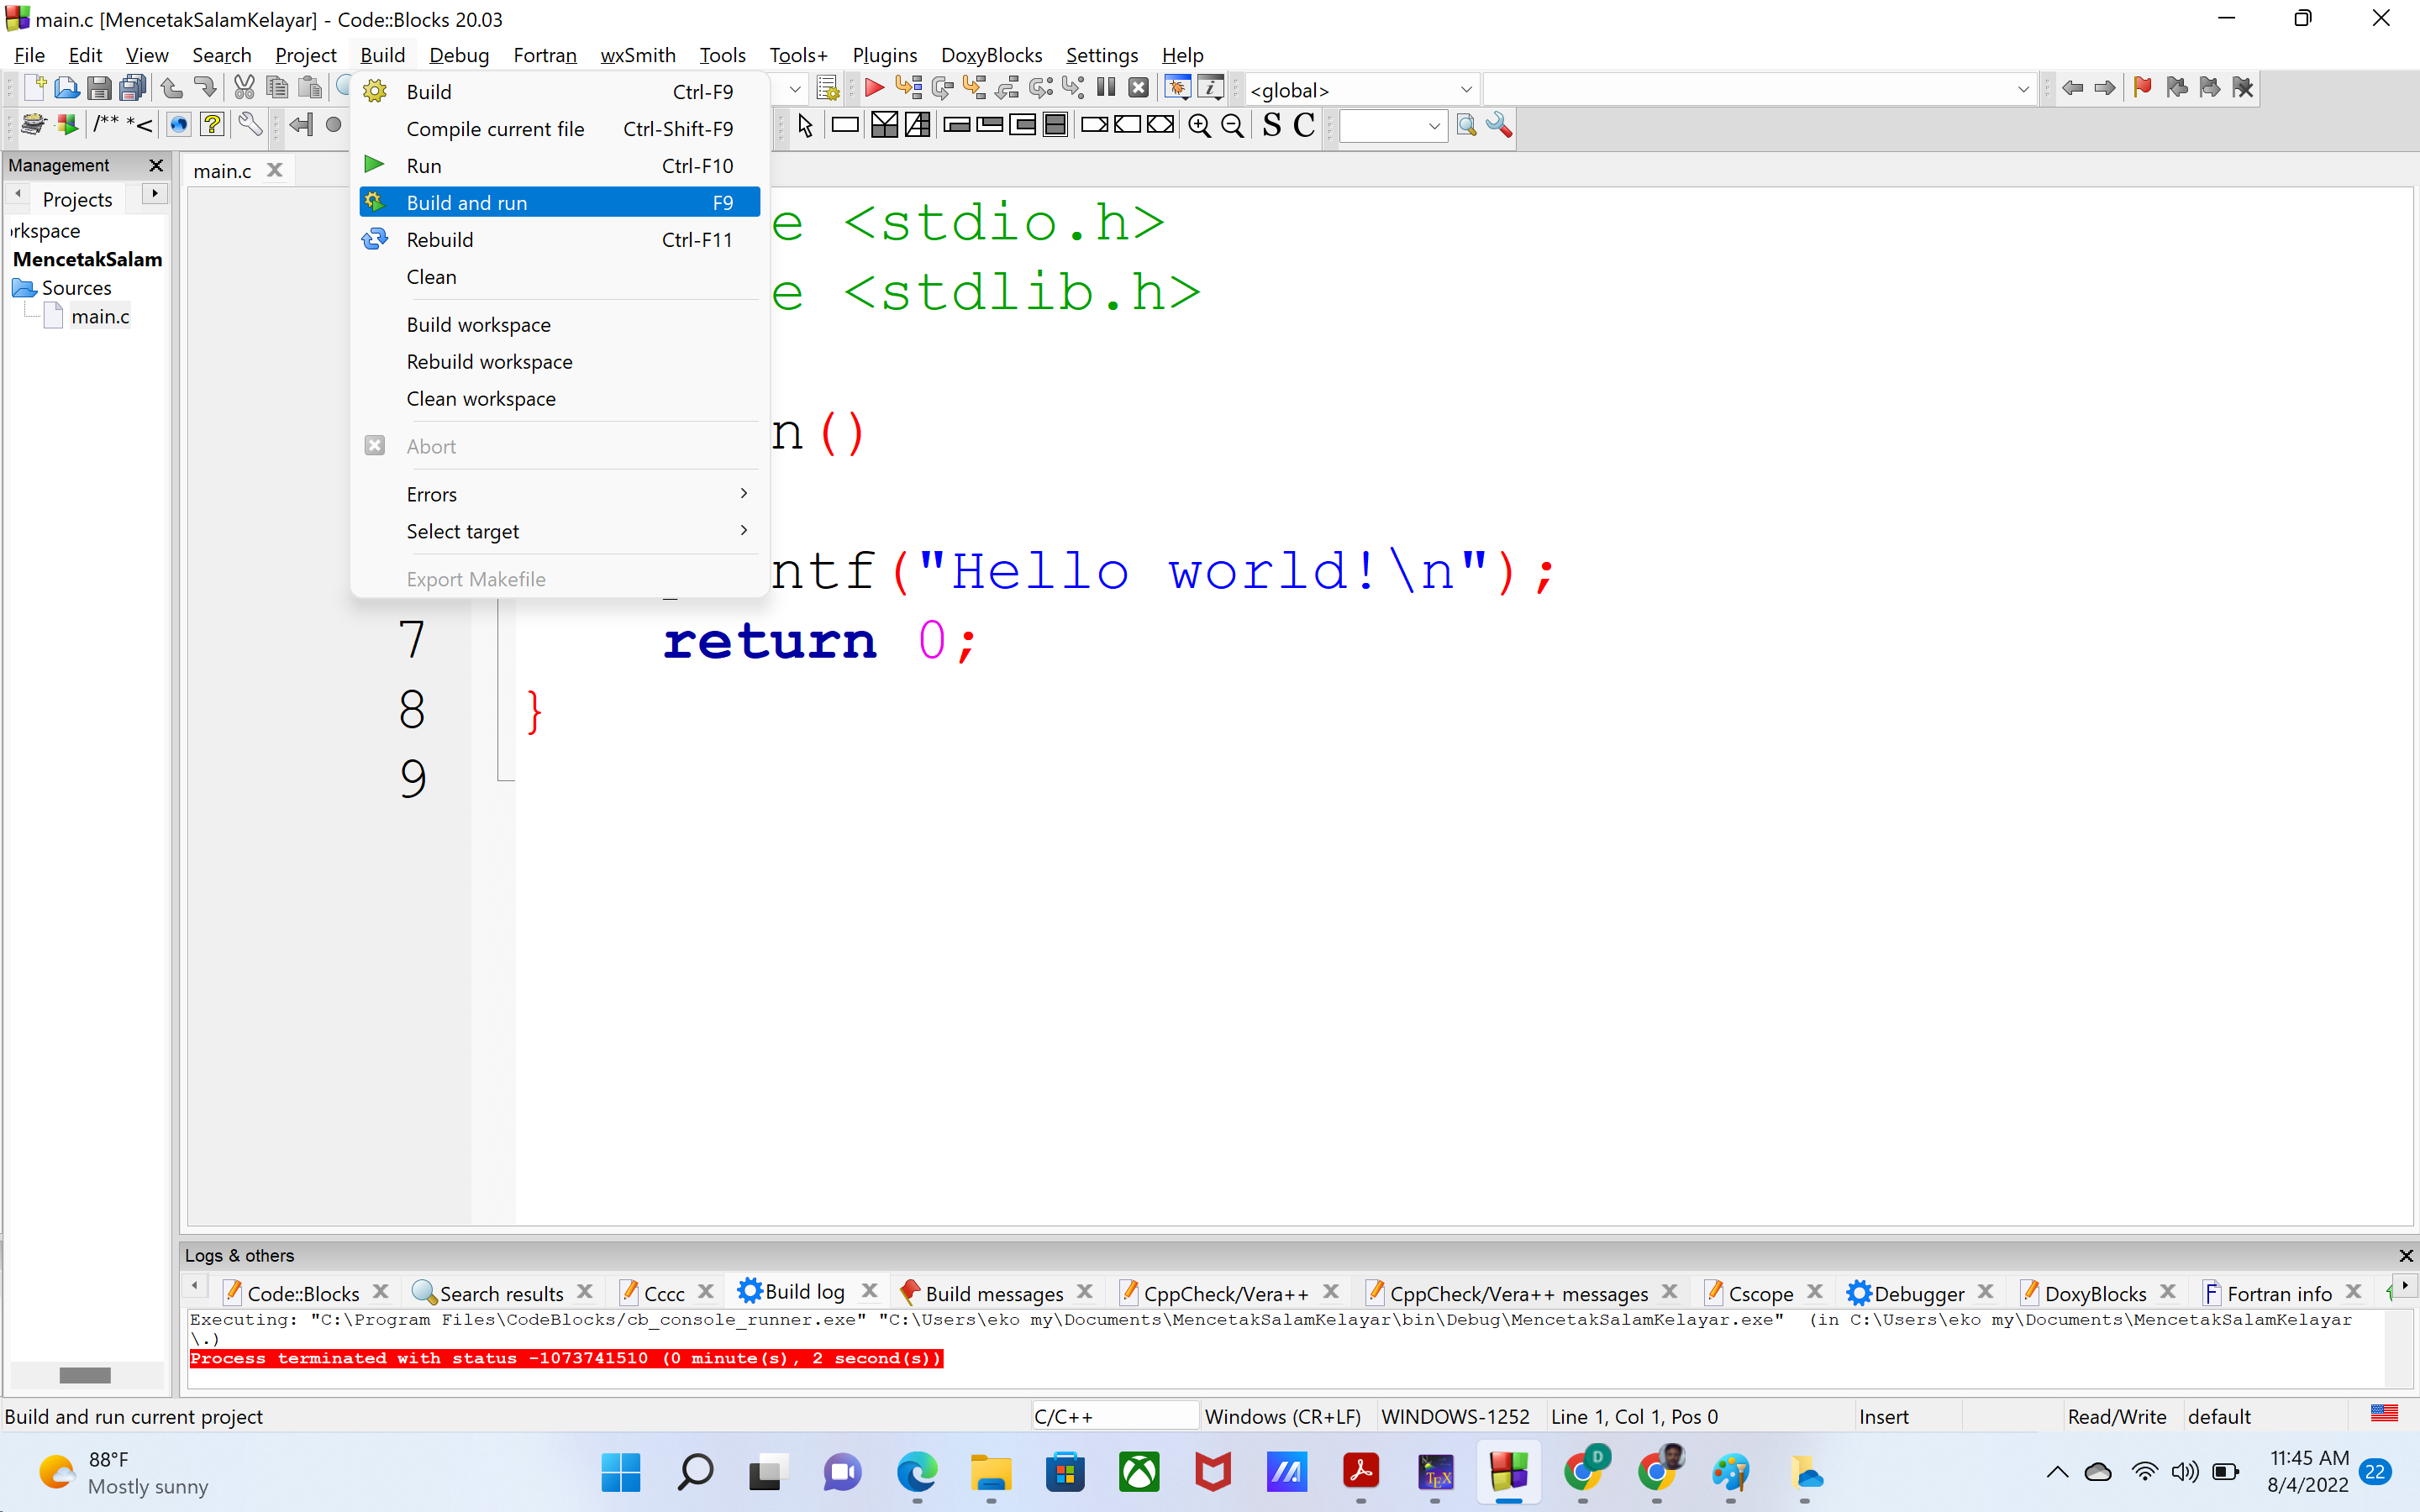
\includegraphics[width=0.7\linewidth]{StrukturProgramC/screenshot009}
	\caption{}
	\label{fig:screenshot009}
\end{figure}
\item The program outputs can be seen on the console.
\begin{figure}[H]
	\centering
	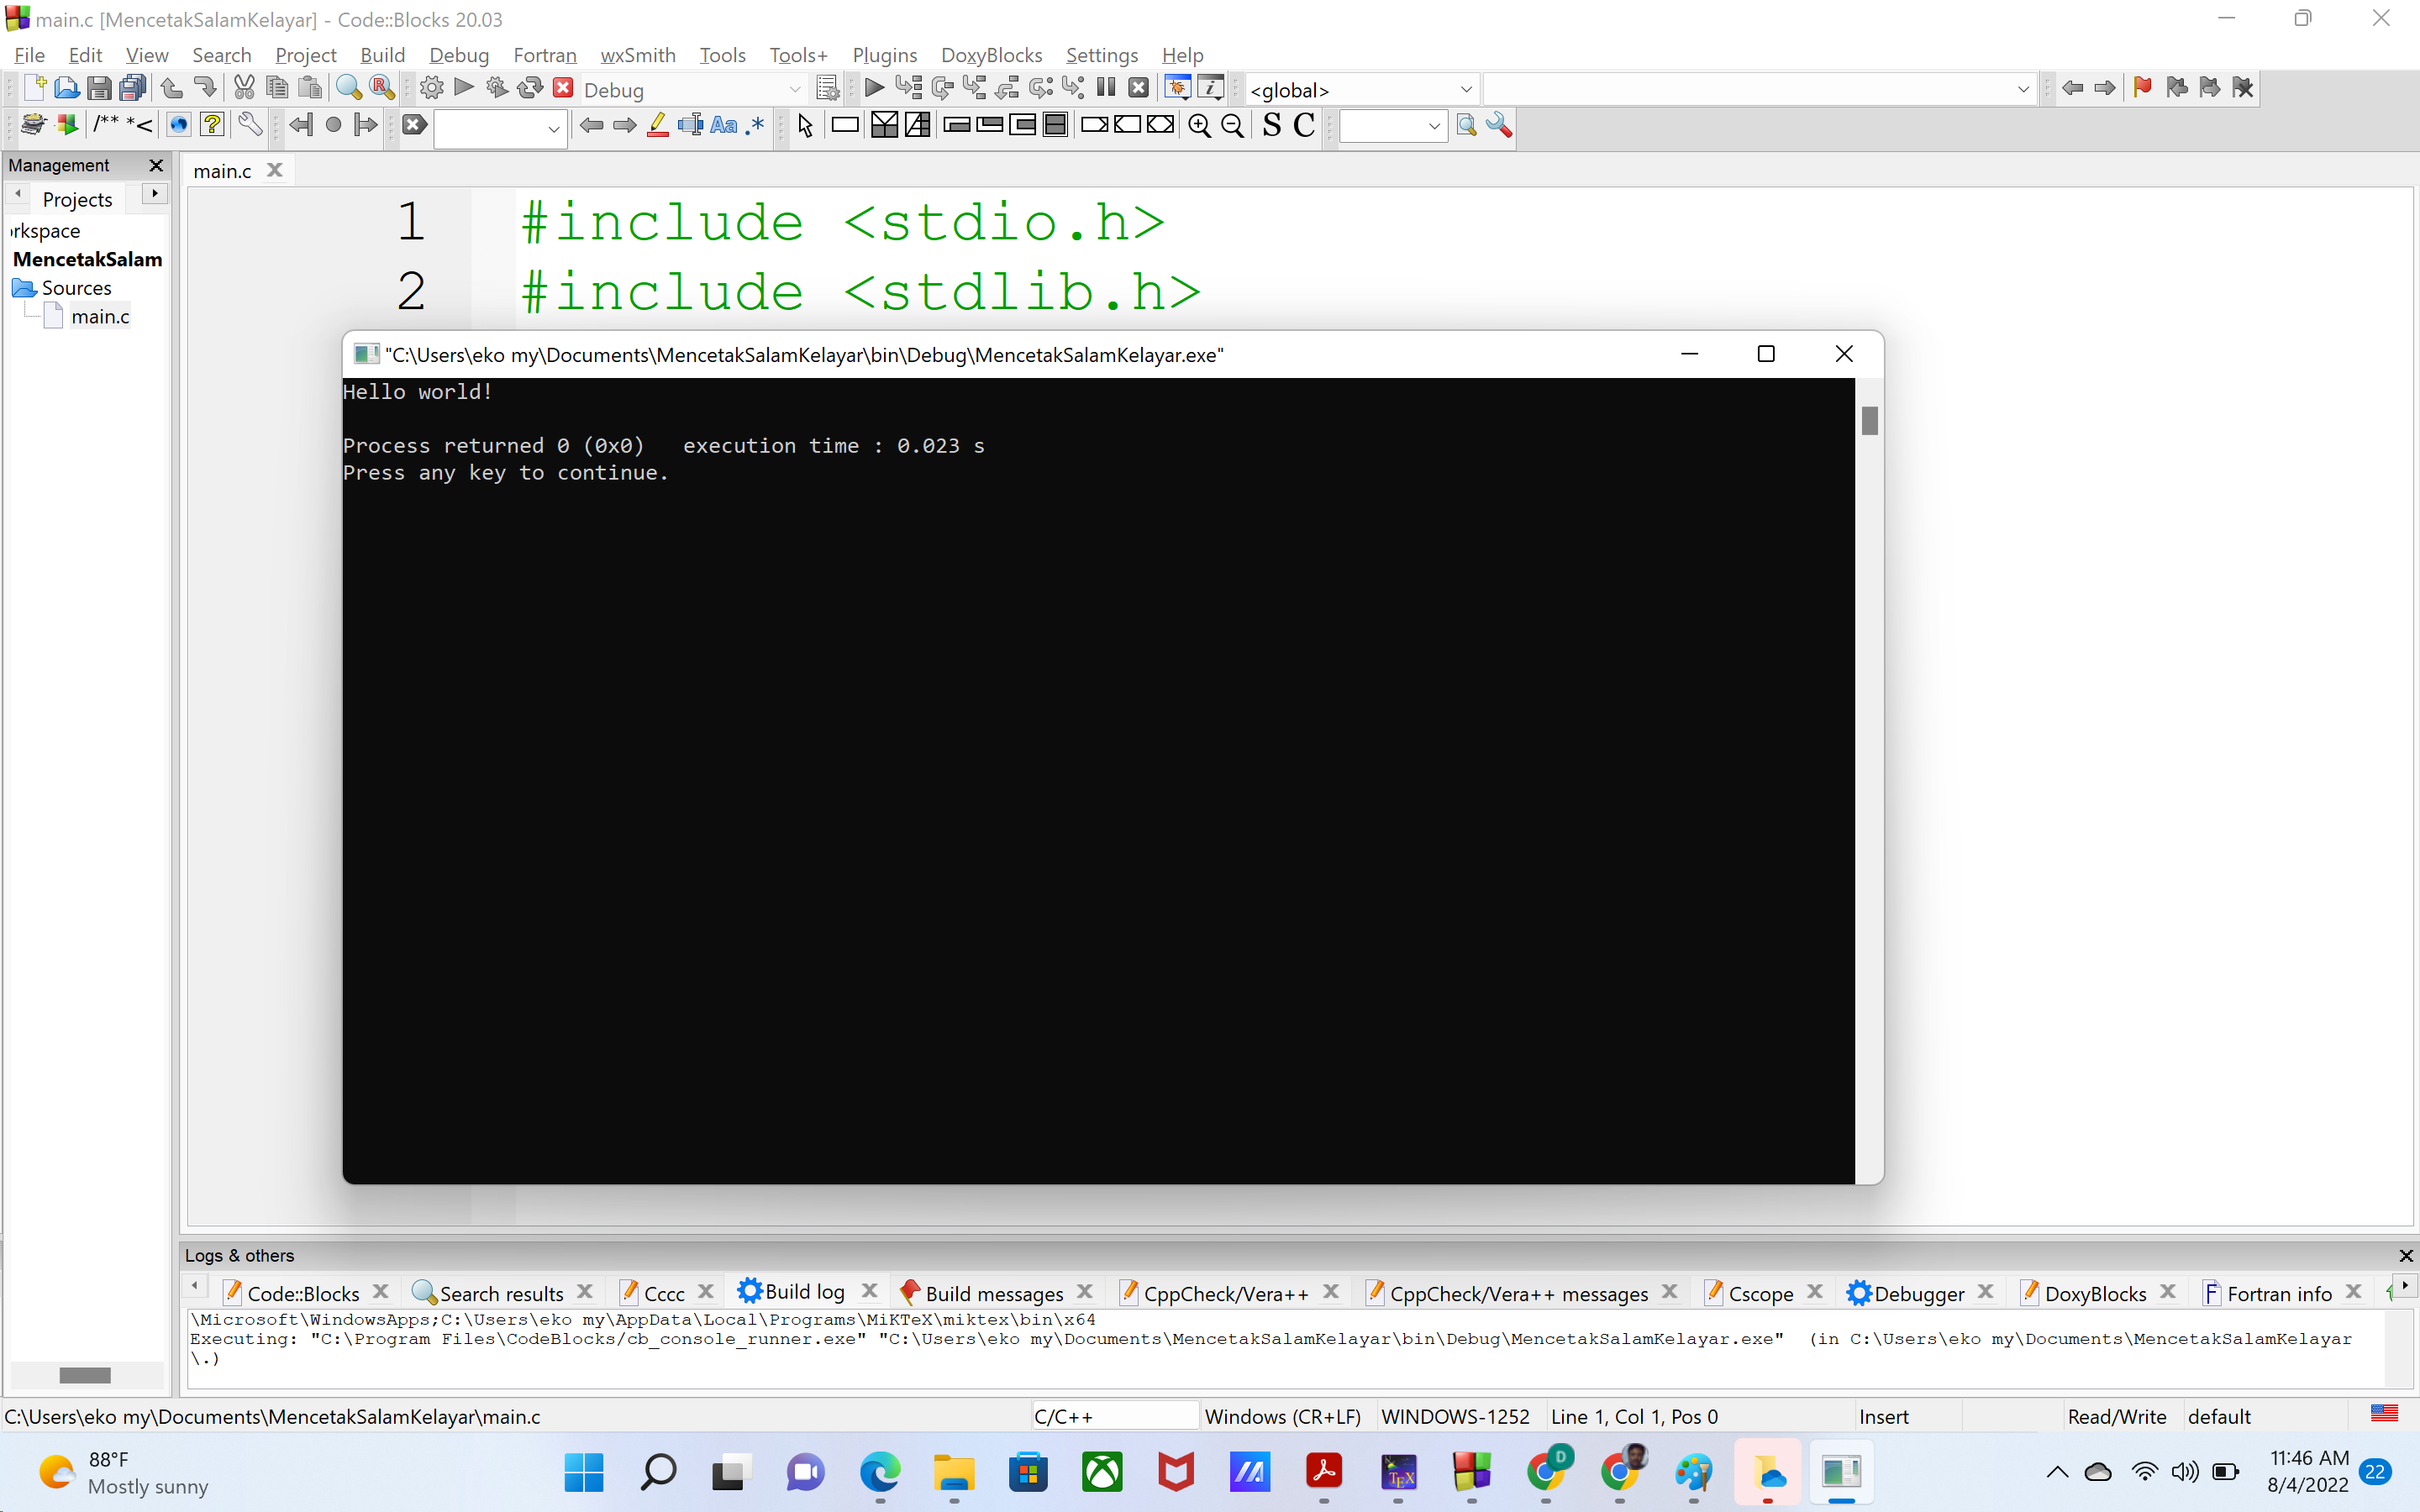
\includegraphics[width=0.7\linewidth]{StrukturProgramC/screenshot010}
	\caption{}
	\label{fig:screenshot010}
\end{figure}
\end{enumerate}

\subsection{Exercise}
Create a project with name HaloDunia and writhe the program like can be seen on figure \ref{fig:screenshot008} but change \verb|Hello World!| with \verb|Halo Dunia!|

%\begin{enumerate}
%	\item  Membuat program untuk menampilkan tulisan ke layar.\\
%	Langkah-langkah
%	\begin{enumerate}
%		\item Buatlah project baru dengan nama :\verb*|MencetakTextKeLayar|
%		\item Ketiklah ulang kode pada Listing \ref{lst:mencetaksalamkelayar}
%		\begin{figure}[H]
%		\begin{lstlisting}[language=c,label=lst:mencetaksalamkelayar,caption=Mencetak Teks Kelayar,captionpos=t]
%			/*Mencetak Text ke layar*/
%			
%			#include <stdio.h>
%			
%			int main()
%			{
%				//Mencetak ke layar
%				printf("Saya belajar  Pemprograman Komputer\n");
%				return 0;
%			}
%			
%		\end{lstlisting}
%	\end{figure}
%	\end{enumerate}
%\end{enumerate}
\section{Structure of C Programming Language}

\begin{lstlisting}[language=c,caption=Contoh program sederhana dalam bahasa C,label=lst:helloworld,captionpos=t]
#include <stdio.h>

int main()
{
	//printing to screen
	printf("Halo Dunia");
	return 0;
}
\end{lstlisting}

Code on Listing \ref{lst:helloworld} is a simple program to print "Halo Dunia" to screen. The following is the explanation what each line of code do in the program.
\begin{itemize}\setlength\itemsep{-0.1em}
	\item [Baris 1 :] \verb|#include <stdio.h>|\\ header file library for input and output functions like \verb|printf()| (the one used on line 6)
	\item[Baris 2 :] Empty line. 
	\item [Baris 3 :] \verb|int main()|\\ The main function. The main function is the first function to be ran when the program starts.
	\item[Baris 4 :] \{ \\Beginning of the \verb|main()| function code block.
	\item[Baris 5 :]\verb|//printing to screen|\\ Comments. Comments are used to explain what the program is doing. Comments are ignored by the program, but helps the reader.
	\item[Baris 6 :]\verb|printf("Halo Dunia");|\\ Printing "Halo Dunia" to the screen.
	\item[Baris 7 :] \verb|return 0;| \\Returning the \verb|main()| function (A function ends when it returns)
	\item [Baris 8 :] \}\\Closing the \verb|main()| function code block.
\end{itemize}
\subsection{Exercise}
Try to swap line 6 and line 7 in Listing \ref{lst:helloworld}. What happened?\\
What if \verb|return 0;| replaced with \verb|return 1;|?




\section{Data Types and Variable}
\subsection{Data Types}
%Pada bahasa C, terdapat beberapa tipe data untuk merepresentasikan data yang berupa bilangan bulat, bilangan real, karakter, string, dan lain-lain. Berikut adalah beberapa tipe data pada C.\\
In C programming language, there are several data types to represent integer, real number, characters, string, and etc.
\begin{center}
    \captionof{table}{Several data types on C \label{tab:tipedata}}
	\begin{tabular}{|l|l|l|}
		\hline
		Data Types & Size         & Description                                         \\ \hline
		int       & 2 or 4 bytes & saves integers                        \\ \hline
		float     & 4 bytes      & saves real numbers to 8 digit behind decimal point. \\ \hline
		double    & 8 bytes      & saves real numbers to 15 digits behind decimal point. \\ \hline
		char      & 1 byte       & saves a character                     \\ \hline
	\end{tabular}
\end{center}
Untuk menampilkan data pada layar, setiap tipe data memiliki format specifier yang dapat digunakan pada formatted string. Berikut adalah format specifier untuk beberapa tipe data.
To show the data on screen, every data type has a format specifier that can be used on formatted string. The following is the format specifier for several data types.
\begin{center}
    \captionof{table}{Format Specifier \label{tab:formatspecifier}}
	\begin{tabular}{|l|l|}
		\hline
		Format Specifier & Data Type   \\ \hline
		\%d or \%i       & int          \\ \hline
		\%f              & float        \\ \hline
		\%lf             & double       \\ \hline
		\%c              & char         \\ \hline
		\%s              & string \\ \hline
	\end{tabular}
\end{center}
%Masih ada lebih banyak tipe data dari pada yang dituliskan pada Tabel \ref{tab:tipedata}. Tipe-tipe data ini dan spesifikasinya bisa ditemukan dengan mudah di internet.
There are still more data types that what was written on Table \ref{tab:tipedata}. These data types and its specification can be found easily on the internet.

\subsection{Variable}
Variable is a place to save data. Declaring a variable can be done in the following.
\begin{lstlisting}[language=c,caption=Deklarasi Variabel C,label=lst:deklarasivariabel,captionpos=t]
DataType VariableName;
\end{lstlisting}
\subsubsection{Arithmatic and Assignment operators}
Assignment operator can be done to variables that have no \verb*|const| or is an l-value variable. Arithmatic operator however can accept both variable with const or not (both l-value and r-value).
The table below shows some arithmatic operators in C.
\begin{center}
    \captionof{table}{Arithmatic Operators in C \label{tab:operatoraritmatika}}
	\begin{tabular}{|c|l|c|}
		\hline
		\multicolumn{1}{|l|}{\textbf{Operator}} & \textbf{Nama} & \multicolumn{1}{l|}{\textbf{Contoh}} \\ \hline
		+  & Addition &\verb|x + y |  \\ \hline
		-  & Substraction &\verb|x = y|   \\ \hline
		*  & Multiplication   & \verb|x * y|  \\ \hline
		/  & Division   & \verb|x/y|  \\ \hline
		\% & Modulo     & \verb|x % y| \\ \hline
	\end{tabular}
\end{center}

The table below shows some assignment operators.
\begin{center}
    \captionof{table}{Assignment Operators \label{tab:operatorpenugasan}}
	\begin{tabular}{|c|c|c|}
		\hline
		\multicolumn{1}{|l|}{Operator} & \multicolumn{1}{l|}{Example}       & \multicolumn{1}{l|}{Equivalent meaning}  \\ \hline
		=   & x = 5   & x = 5      \\ \hline
		+=  & x += 3  & x = x + 3  \\ \hline
		-=  & x -= 3  & x = x - 3  \\ \hline
		*=  & x *= 3  & x = x * 3  \\ \hline
		/=  & x /= 3  & x = x / 3  \\ \hline
		\%= & x \%= 3 & x = x \% 3 \\ \hline
		\&= & x \&= 3 & x = x \& 3 \\ \hline
		|=  & x |= 3  & x = x | 3  \\ \hline
		\textasciicircum{}=            & x \textasciicircum{}= 3           & x = x \textasciicircum 3           \\ \hline
		\textgreater{}\textgreater{}=  & x \textgreater{}\textgreater{}= 3 & x = x \textgreater{}\textgreater 3 \\ \hline
		\textless{}\textless{}=        & x \textless{}\textless{}= 3       & x = x \textless{}\textless 3       \\ \hline
	\end{tabular}
\end{center}
There is also "shorthands" for some assignments operator like \verb*|x+=1| and \verb*|x-1| which are \verb*|++| and \verb*|--| that is called increment and decrement respectively.
These shorthands are used like the following.
\begin{verbatim}
    x++;
    x--;
    ++x;
    --x;
\end{verbatim}


\subsection{Exercise}
\begin{lstlisting}[language=c,caption=Using assignment operator on const variable,label=lst:constassignment,captionpos=t]
#include <stdio.h>
int main()
{
    //deklarasi variabel const
    const int x=0;
    x=1;
	return 0;
}
\end{lstlisting} 
Try to compile the program in Listing\ref{lst:constassignment}, what happened?










\section{Output and Input}

\subsection{printf()}
\verb*|printf| is a function in C that is used to print formatted string. % digunakan untuk mencetak string  ke output yang dilengkapi dengan format specifirer yang dimulai dengan \verb*|%| pada string.
You can use format specifier within the formatted string to outputs your variables.

\begin{verbatim}
	printf(const char *format,v1,v2,..,vn)
\end{verbatim}

%format specifier untuk beberapa tipe data dapat dilihat pada Tabel \ref{tab:formatspecifier}
The format specifier for each data types can be seen on Table \ref{tab:formatspecifier}


\begin{description}
	\item[Contoh \thesection.1]  Printing text to the screen.
	\begin{lstlisting}[language=c,caption = Mencetak Tulisan "Pemprograman C Ke layar,captionpos=t]
		#include <stdio.h>    
		int main()
		{ 
			// Printting the text written within the " symbol
			printf("C Programming");
			return 0;
		}
	\end{lstlisting}
	\begin{itemize}
		%\item Seluruh program C harus berisi fungsi main() tempat program memulai menjalankan kode. 
		\item All C program must have main() function where the program needs to run the code.
		%\item Fungsi \verb*|printf()| adalah library untuk mengirim output yang telah diformat ke layar.  Fungsi \verb*|printf()|  mencetak string dalam tanda dua tanda petik. 
		\item \verb*|printf()| function is a function from stdio.h library. This function outputs the string inside the symbol " to the screen.
		\item \verb*|return 0;| statement in the \verb*|main()| function tells the program to exit.
	\end{itemize}
	\item [Contoh \thesection.2] Printing integer. 
	\begin{lstlisting}[language=c,captionpos=t]
		#include <stdio.h>
		int main()
		{
			int testInteger = 5;
			printf("Number = %d", testInteger); // <- %d format string
			return 0;
		}
	\end{lstlisting}
	
	
	%Pada contoh ini digunakan format spcifier \verb*|%d| untuk mencetak tipe data \verb*|int|. \verb*|%d| pada tex akan digantikan oleh isi dari \verb*|testInteger|. 
	The code above uses the format specifier \verb*|%d| to prints \verb*|int| data type. The \verb*|%d| part of the string will be replaced with the value of \verb*|testInteger|.

	\item[Contoh \thesection.3] Output real numbers (float or double)
	\begin{itemize}\label{eq:LuasSegitiga}
		\item \verb|Base|  : using \verb|float| data type.
		\item \verb|Height|: using \verb|float| data type.
		\item \verb|Area|  : using \verb|float| data type.
		\item Triangle area formula: 
		\begin{equation}
			Luas = \frac{1}{2} \times Alas \times Tinnggi
		\end{equation}
	\end{itemize}
	\begin{lstlisting}[language=c,captionpos=t]
		#include <stdio.h>
		
		int main()
		{
			// declare the variables
			float Base;
			float Height;
			float Area;
			// Initialize the values
			Base = 10;
			Height = 5;
			// Calculate the area
			Area = 0.5*Base*Height;
			//Print the area to the screen
			printf("Area = %f",Area);
			return 0;
		}
		
	\end{lstlisting}
	
	Explanation:
	\begin{description}
		\item[Line 6-8] Declaring the variables needed to save the data about the triangle. % \verb|Alas|, \verb|Tinggi| dan \verb|Luas| bertipe data \verb|float| untuk menyimpan data parameter luas segitiga.
		\item[Line 10 dan 11] Giving values to the variables %Memberi nilai ke Variabel \verb|Alas|=10 dan \verb|Tinggi|=5
		\item[Line 13] Calculate the area according to the formula %Menghitung luas alas sesuai dengan persamaan \ref{eq:LuasSegitiga}
		\item[Line 15] Prints the area with printf and \verb|%f| format specifier %Mencetak \verb|Luas| ke layar dengan menggunakan perintah \verb|printf|.
	\end{description}
\end{description}

.\section{scanf}
%Fungsi  \verb*|scanf(const char *format, ...)| membaca input dengan format.
\verb*|scanf(const char *format, ...)| reads input according to the format string.

\begin{enumerate}
	\item Syntax 
	\begin{verbatim}
		scanf(const char *format, ...)
	\end{verbatim}
	\item Parameter \\
	Format string in C consist of one or more whitespace, non-whitespace, and format specifiers.
	%format string pada C yang terdiri dari satu atau lebih yang terdiri dari \\
	%Karakter Whitespace,Karakter Non-whitespace  dan  Format specifiers. 
	\item Return Value \\
	%Ketika berhasil maka fungsi mengembalikan jumlah item dari argumen yang berhasil di baca.
	The function will return the number of arguments it has sucessfully read.
	
\end{enumerate}

\begin{description}
	\item  [\thesection.1] Calculating the area of an triangle  with the base \verb*|Alas|   dan height \verb*|Tinggi| is inputted from keyboard 
	\begin{lstlisting}[language=c]
#include <stdio.h>

int main()
{
	float Alas ,Tinggi,Luas;
	
	printf("Calculating the area of an triangle\n");
	printf("\nEnter the base length= ");
	scanf("%f",&Alas);
	printf("\nEnter the height=");
	scanf("%f",&Tinggi);
	Luas = 0.5*Alas *Tinggi;
	printf("Triangle area = %.2f", Luas);
	return 0;
}
	\end{lstlisting}
\begin{figure}[H]
	\centering
	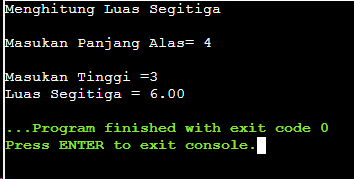
\includegraphics[width=0.5\linewidth]{StrukturProgramC/screenshot0005.png}
	\caption{}
	\label{fig:screenshot0005}
\end{figure}

\begin{description}
	\item [Line 9]\verb|scanf("%f",&Alas);| ask for the input for the the triangle base
	\item [Line 11]\verb|scanf("%f",&Tinggi);| ask for the input for the triangle height
	\item [Line 13]\verb|printf("Triangle Area = %.2f", Luas);|, The \verb|.2| in \verb|%.2f| tells the program to outputs only 2 digits after the decimal point.%menandakan bahwa hanya 2 angka di belakang koma(decimal point) yang perlu dicetak.
\end{description}

	\item[Contoh \thesection.2] Program to input name and email.\\
	%Pada contoh ini dipelajari bagaimana cara menginputkan string atau text dari keyboard dan mencetak kelayar. Input dari contoh program ini ada dua yang terdiri dari \verb|snama| dan \verb|sAlamatEmail|. Oleh karena text berisi banyak karakter maka masing-masing variabel dideklarasikan sebagai kumpulan karakter dengan jumlah karakter untuk sNama=20 dan sAlamatEmail=30. 
	This example shows how to input string or text from keyboard and outputs it on the screen. Input from this program consist of \verb|sName| and \verb|sEmail|.
	\begin{figure}[H]
	\begin{lstlisting}[language=c]
		#include <stdio.h>
		
		int main () 
		{
			char sName[20], sEmail[30];
			
			printf("Insert Name: ");
			scanf("%19s", sName);
			
			printf("Insert Email : ");
			scanf("%29s", sEmail);
			
			printf("Name : %s\n", sName);
			printf("Email:%s", sEmail);
			return(0);
		}
	\end{lstlisting}
\end{figure}
\end{description}


\subsection{Escape Sequence}
%Escape Sequence adalah urutan karakter yang digunakan untuk memformat output dan tidak ditampilkan ketika dicetak ke layar. Setiap karakter mempunyai fungsi tertentu. 
Some characters can't be written on the format string because they are used to format the outputs.
So, to outputs those special characters we use escape sequences.

\begin{table}[H]
	\centering
	\captionof{table}{Escape Sequence \label{tab:escapesequence}}
	\begin{tabular}{|l|l|l|}
		\hline
		Escape sequence & What it will output &  \\ \hline
		\textbackslash{}a & bell, alarm &  \\ \hline
		\textbackslash{}b & Backspace &  \\ \hline
		\textbackslash{}f & Ganti halaman &  \\ \hline
		\textbackslash{}n & Ganti baris &  \\ \hline
		\textbackslash{}r & Carriage return &  \\ \hline
		\textbackslash{}t & tab horisontal&  \\ \hline
		\textbackslash{}v & tab vertikal &  \\ \hline
		\textbackslash{}' & Petik tunggal  &  \\ \hline
		\textbackslash{}" & Petik Ganda &  \\ \hline
		\textbackslash{}? & Tanda tanya &  \\ \hline
		\textbackslash{}\textbackslash{} & Backslash &  \\ \hline
	\end{tabular}
\end{table}

\begin{description}
	\item[Example \thesection.1] Changing line with the escape sequence \verb*|\n|.
	\begin{lstlisting}
#include <stdio.h>

int main() 
{
	printf("Halo \nSaya sedang belajar bahasa C.\ndan ini sangat menyenangkan!");
	return 0;
}
	\end{lstlisting}
\begin{figure}[H]
	\centering
	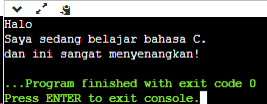
\includegraphics[width=0.5\linewidth]{StrukturProgramC/screenshot0006.png}
	\caption{}
	\label{fig:screenshot0006}
\end{figure}

\item[Contoh \thesection.1] Using escape sequence \verb*|\t| setting the tab.
\begin{lstlisting}[language=c]
#include <stdio.h>
int main(void)
{
	printf("Nama \t\t: Rahmad Rahardi\n");
	printf("Alamat \t\t: Bendungan Hilir Jakarta\n");
	printf("Tempat Lahir \t: Jakarta\n");
	printf("Tanggal Lahir \t: 30 Pebruari 2000\n");
	
	return (0);
}
\end{lstlisting}
\begin{figure}[H]
	\centering
	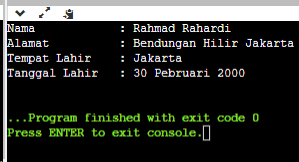
\includegraphics[width=0.5\linewidth]{StrukturProgramC/screenshot0007.png}
	\caption{}
	\label{fig:screenshot0007}
\end{figure}
\end{description}

\subsection{Latihan}
Cobalah buat suatu program yang dapat menerima input berupa nama dan NRP kemudian menampilkannya pada layar.






\chapter{Conditional Instruction}

\section{Goals}
\begin{itemize}
%    \setlength\itemsep{0.5em}
	%\item Mahasiswa mengenal dan mampu menggunakan ekspresi-ekspresi logika dan perbandingan pada bahasa pemrograman C
	\item Students know and able to utilize logical and comparison expression in C programming language.
	%\item Mahasiswa mengenal dan mampu menggunakan syntax-syntax percabangan pada bahasa pemrograman C
	\item Students know and able to utilize conditional instruction sytaxes in C programming language.
\end{itemize}


\section{Logical and Comparison Expression}

\subsection{Comparison Expression}
Berikut adalah operator-operator yang digunakan pada suatu ekspresi perbandingan
The following are the operators used in comparison expressions.
\begin{center}
    \captionof{table}{Comparison Operators \label{tab:operatorcomp}}
	\begin{tabular}{|c|l|c|}
		\hline
		Operator        & Name                                   & \multicolumn{1}{l|}{Example Expression} \\ \hline
		==              & Equals	                             & x == y                       \\ \hline
		!=              & Not Equals 	                         & x != y                       \\ \hline
		\textgreater{}  & Greater than                           & x \textgreater y             \\ \hline
		\textless{}     & Lesser than                            & x \textless y                \\ \hline
		\textgreater{}= & Greater or Equal than				 	 & x \textgreater{}= y          \\ \hline
		\textless{}=    & Lesser or Equal than           		 & x \textless{}= y             \\ \hline
	\end{tabular}
\end{center}

%Suatu ekspresi perbandingan akan mengembalikan nilai berupa \verb|true| atau \verb|false| yang ditandakan dengan nilai 0 atau 1.
A Comparison Expression will return boolean value \verb|true| or \verb|false| which is also represented with the value 1 or 0.
%Sebagai contoh:
As example:
\begin{verbatim}
    printf("%d",0>1); // will output 0 to the screen
    printf("%d",0<1); // will output 1 to the screen 
\end{verbatim}

\subsection{Logical Expression}
Berikut adalah operator-operator logika yang digunakan pada suatu ekspresi logika
The following are the logical operators used on a Logical Expression
\begin{center}
    \captionof{table}{Logical Expression \label{tab:operatorlogic}}
	\begin{tabular}{|c|l|c|}
		\hline
		Operator & \multicolumn{1}{c|}{Name} & Example Expression \\ \hline
		$\&\&$    &  AND                & $x<5\; \&\& \;x<10$\\ \hline
		$||$    &  OR                 & $x < 5\; ||\; x < 4  $     \\ \hline
		$!$        & NOT                & $!(x <5 \&\& x < 10) $\\ \hline
	\end{tabular}
\end{center}
%Sama seperti ekspresi perbandingan, ekspresi logika akan mengembalikan nilai berupa true atau false
Like comparison expression, logical expression will return boolean values.


\section{If statement}
\verb*|if| statement is used to decide which block of code to be executed if the condition is true.
%digunakan untuk menentukan blok kode C yang dijalankan apabila ekspresi kondisi bernilai benar (TRUE),
\begin{verbatim}
// Block of code before if
if (Condition) 
{
 // Block of code to be executed if the condition is true.
}
// block of code after if
\end{verbatim}
Sebagai contoh, perhatikan program berikut
As example, look at the following code 
\begin{lstlisting}[language=c,caption = If statement example,label=lst:ifexample01]
	include <stdio.h>
	
	int main()
	{
		//Deklarasi variabel 
		int uangSaya,hargaRoti;
		uangSaya = 5000;
		hargaRoti = 10000;
		
		if (uangSaya>=hargaRoti)
		{
		    printf("saya bisa beli roti\n");
		}
		printf("hehe");
		return 0;
	}
\end{lstlisting}                        
This program outputs
\begin{verbatim}
    hehe
\end{verbatim}
If line 7 changed to \verb|uangSaya=10000|, the outputs of the program would be
%Jika baris ke 7 diganti dengan \verb|uangSaya=10000| maka output dari program ini akan menjadi
\begin{verbatim}
    saya bisa beli roti
    hehe
\end{verbatim}

\section{If-else statement}
Statement else digunakan untuk menentukan blok kode yang di jalankan apabila kondisi salah. 
Else statement is used to decide the block of code to be executed if the condition is false.
\begin{verbatim}
// Block of code before if
if (Condition) 
{
	// Block of code to be executed if the condition is true
} else
{
	// Block of code to be executed if the condition is false
}
// Block of code after if-else statement
\end{verbatim}
%Berikut contoh penggunaan if-else
The following is an example of using if-else statement:
\begin{lstlisting}[language=c,caption = if-else example,label=lst:ifelseexample01]
	include <stdio.h>
	
	int main()
	{
		//Deklarasi variabel 
		int uangSaya,hargaRoti;
		uangSaya = 5000;
		hargaRoti = 10000;
		
		if (uangSaya>=hargaRoti)
		{
		    printf("saya bisa beli roti\n");
		}
		else
		{
	        printf("saya tidak bisa beli roti\n");	
		}
		printf("hehe");
		return 0;
	}
\end{lstlisting}                        
The output of the program is
\begin{verbatim}
    saya tidak bisa beli roti
    hehe
\end{verbatim}
%Jika baris ke 7 diganti dengan \verb|uangSaya=10000| maka output dari program ini akan menjadi
If line 7 changed to \verb|uangSaya=10000|, the outputs of the program would be
\begin{verbatim}
    saya bisa beli roti
    hehe
\end{verbatim}
\section{Statement if-else if}
Statement \verb|else if| digunakan untuk menjalankan blok kode apabila kondisi statement \verb|if| atau \verb|else if| sebelumnya bernilai salah.
The \verb|else if| statement is used to run a block of code when the condition in \verb|if| or the previous \verb|else if| is false.
\begin{verbatim}
	// block of code before if
    if (Condition1)
    {
	  /* block of code to be executed if Condition1
	  is true*/
    }
    else if (Condition2)
    {
	  /* block of code to be executed if Condition1 is false
	  and Condition2 is true */
    }
    else if (Condition3)
    {
	  /* Block of code to be executed when
	  Condition1 and Condition2 is false and
	  Condition3 is true*/
    }
    ...
    else if (ConditionN)
    {
	  /* Block of code to be executed when
	  Condition1 to ConditionN-1 is false and
	  ConditionN is true*/
    }
    else
    {
	  /* Block of code to be executed when
	  Condition1 to ConditionN is false*/
    }
	// Block of code after if
\end{verbatim}
Berikut contoh penggunaan if-else if
\begin{lstlisting}[language=c,caption = if-else if example,label=lst:ifelseifexample01]
	include <stdio.h>
	
	int main()
	{
		//Deklarasi variabel 
		int uangSaya,hargaRoti;
		uangSaya = 5000;
		hargaRoti = 10000;
		
		if (uangSaya>hargaRoti)
		{
		    printf("saya bisa beli roti\n");
		}
		else if(uangSaya==hargaRoti)
		{
		    printf("saya bisa beli roti tapi uang saya akan langsung habis\n");
		}
		else
		{
	        printf("saya tidak bisa beli roti\n");	
		}
		printf("hehe");
		return 0;
	}
\end{lstlisting}                        
The output of this program is
\begin{verbatim}
    saya tidak bisa beli roti
    hehe
\end{verbatim}
%Jika baris ke 7 diganti dengan \verb|uangSaya=10000| maka output dari program ini akan menjadi
If line 7 changed to \verb|uangSaya=10000|, the output of the program would be
\begin{verbatim}
    saya bisa beli roti tapi uang saya akan langsung habis
    hehe
\end{verbatim}
%Jika baris ke 7 diganti dengan \verb|uangSaya=12000| maka output dari program ini akan menjadi
If line 7 changed to \verb|uangSaya=12000|, the output of the program would be
\begin{verbatim}
    saya bisa beli roti
    hehe
\end{verbatim}

\section{Nested if}
%nested if merupakan konsep di mana di dalam suatu blok if terdapat statement if.
Nested if is when there is a conditional statements within a block of code inside the conditional statement
\begin{verbatim}
// Block of code before if
if (Condition1) 
{
    if (Condition2)
    {
        // do something
    }
    else
    {
        // do another thing
    }
} 
else
{
    // do something else
}
\end{verbatim}

%Berikut contoh penggunaan nested if
Below is an example of using nested if

\begin{lstlisting}[language=c,caption = nested if example,label=lst:nestedifexample01]
	include <stdio.h>
	
	int main()
	{
		// Declare the variables
		int myMoney,breadPrice,friendsMoney;
		myMoney = 5000;
		breadPrice = 10000;
		friendsMoney = 42069;
		
		
		if (myMoney>breadPrice)
		{
		    printf("I can buy bread\n");
		}
		else if(myMoney==breadPrice)
		{
		    printf("I can buy bread but I will ran out of money\n");
		}
		else
		{
		    if(friendsMoney+myMoney >= breadPrice)
		    {
		        printf("I can buy bread if I borrow my friend money\n"); 
		    }
		    else
		    {
	            printf("I can't buy bread\n");	
		    }
		}
		printf("hehe");
		return 0;
	}
\end{lstlisting}


\section{Exercise}
%Coba buat program yang menerima input 3 buah bilangan bulat A, B, dan C. Outputkanlah 3 bilangan bulat itu ke layar dengan urutan paling kecil ke paling besar. Lakukanlah ini dengan menggunakan statement if, if else, if else if, atau nested if.
Try to make a program that receives 3 integer input A, B, and C. Then outputs those 3 integers to the screen sorted from smallest to largest. Do this only using conditional statements.

%/KontrolAliranProgram}
\section{Goals}
\begin{itemize}
    \item Mahasiswa mengenal dan mampu menggunakan ekspresi-ekspresi logika dan perbandingan pada bahasa pemrograman C
    \item Mahasiswa mengenal dan mampu menggunakan syntax-syntax percabangan pada bahasa pemrograman C
    \item Mahasiswa dapat mengenal dan menggunakan perulangan while pada bahasa C
    % \item Students are able to use while-loop on C
    \item Mahasiswa dapat mengenal dan menggunakan perulangan do-while pada bahasa C
    % \item Students are able to use do-while loop on C
    \item Mahasiswa dapat mengenal dan menggunakan perulangan for pada bahasa C
    % \item Students are able to use for loop on C
    \item Mahasiswa dapat mengenal dan menggunakan  array dimensi satu maupun multidimensi.
    % \item Students are able to use one dimensional or multidimensional array
    \item Mahasiswa mampu memanfaatkan perulangan untuk mengolah data pada array.
    % \item Students are able to use loops to process data on arrays
\end{itemize}
\section{Ekspresi Logika dan Perbandingan}
\subsection{Ekspresi Perbandingan}
Berikut adalah operator-operator yang digunakan pada suatu ekspresi perbandingan
% The following are the operators used in comparison expressions.
\begin{center}
    \captionof{table}{Operator Perbandingan \label{tab:operatorcomp}}
	\begin{tabular}{|c|l|c|}
		\hline
		Operator        & Nama                                 & \multicolumn{1}{l|}{Contoh Ekspres} \\ \hline
		==              & Sama Dengan	                             & x == y                       \\ \hline
		!=              & Tidak Sama Dengan	                         & x != y                       \\ \hline
		\textgreater{}  & Lebih Dari                          & x \textgreater y             \\ \hline
		\textless{}     & Kurang Dari                           & x \textless y                \\ \hline
		\textgreater{}= & Lebih Dari Sama Dengan			 	 & x \textgreater{}= y          \\ \hline
		\textless{}=    & Kurang Dari Sama Dengan           		 & x \textless{}= y             \\ \hline
	\end{tabular}
\end{center}

Suatu ekspresi perbandingan akan mengembalikan nilai berupa \verb|true| atau \verb|false| yang ditandakan dengan nilai 0 atau 1.
% A Comparison Expression will return boolean value \verb|true| or \verb|false| which is also represented with the value 1 or 0.
Sebagai contoh:
As example:
\begin{verbatim}
    printf("%d",0>1); // Akan Mencetak 0 ke layar
    printf("%d",0<1); // Akan Mencetak 1 ke layar 
\end{verbatim}

\subsection{Ekspresi Logika}
Berikut adalah operator-operator logika yang digunakan pada suatu ekspresi logika
% The following are the logical operators used on a Logical Expression
\begin{center}
    \captionof{table}{Ekspresi Logika \label{tab:operatorlogic}}
	\begin{tabular}{|c|l|c|}
		\hline
		Operator & \multicolumn{1}{c|}{Nama} & Contoh Ekspresi \\ \hline
		$\&\&$    &  AND                & $x<5\; \&\& \;x<10$\\ \hline
		$||$    &  OR                 & $x < 5\; ||\; x < 4  $     \\ \hline
		$!$        & NOT                & $!(x <5 \&\& x < 10) $\\ \hline
	\end{tabular}
\end{center}
Sama seperti ekspresi perbandingan, ekspresi logika akan mengembalikan nilai berupa true atau false
% Like comparison expression, logical expression will return boolean values.

\section{Percabangan}
\subsection{Pernyataan If}
% \verb*|if| statement is used to decide which block of code to be executed if the condition is true.
\verb*|if| digunakan untuk menentukan blok kode C yang dijalankan apabila ekspresi kondisi bernilai benar (TRUE),
\begin{verbatim}
// Block of code before if
if (Condition) 
{
 // Blok kode yang akan dieksekusi jika kondisinya benar(True).
}
// Blok kode setelah if
\end{verbatim}
Sebagai contoh, perhatikan program berikut
% As example, look at the following code 
\begin{lstlisting}[language=c,caption =Contoh Pernyataan If,label=lst:ifexample01]
	include <stdio.h>
	
	int main()
	{
		//Deklarasi variabel 
		int uangSaya,hargaRoti;
		uangSaya = 5000;
		hargaRoti = 10000;
		
		if (uangSaya>=hargaRoti)
		{
		    printf("saya bisa beli roti\n");
		}
		printf("hehe");
		return 0;
	}
\end{lstlisting}                        
Keluaran program ini
\begin{verbatim}
    hehe
\end{verbatim}
% If line 7 changed to \verb|uangSaya=10000|, the outputs of the program would be
Jika baris ke 7 diganti dengan \verb|uangSaya=10000| maka output dari program ini akan menjadi
\begin{verbatim}
    saya bisa beli roti
    hehe
\end{verbatim}

\subsection{Pernyataan If-else}
Pernyataan else digunakan untuk menentukan blok kode yang di jalankan apabila kondisi salah. 
% Else statement is used to decide the block of code to be executed if the condition is false.
\begin{verbatim}
// Blok kode sebelum if
if (Condition) 
{
	// Blok kode yang akan dieksekusi jika kondisinya benar
} else
{
	// Blok kode yang akan dieksekusi jika kondisinya salah
}
// Blok kode setelah pernyataan if-else
\end{verbatim}
Berikut contoh penggunaan if-else
% The following is an example of using if-else statement:
\begin{lstlisting}[language=c,caption = if-else example,label=lst:ifelseexample01]
	include <stdio.h>
	
	int main()
	{
		//Deklarasi variabel 
		int uangSaya,hargaRoti;
		uangSaya = 5000;
		hargaRoti = 10000;
		
		if (uangSaya>=hargaRoti)
		{
		    printf("saya bisa beli roti\n");
		}
		else
		{
	        printf("saya tidak bisa beli roti\n");	
		}
		printf("hehe");
		return 0;
	}
\end{lstlisting}                        
Keluaran program adalah sebagai berikut
\begin{verbatim}
    saya tidak bisa beli roti
    hehe
\end{verbatim}
Jika baris ke 7 diganti dengan \verb|uangSaya=10000| maka output dari program ini akan menjadi
% If line 7 changed to \verb|uangSaya=10000|, the outputs of the program would be
\begin{verbatim}
    saya bisa beli roti
    hehe
\end{verbatim}

\subsection{Pernyataan if-else if}
Statement \verb|else if| digunakan untuk menjalankan blok kode apabila kondisi statement \verb|if| atau \verb|else if| sebelumnya bernilai salah.
% The \verb|else if| statement is used to run a block of code when the condition in \verb|if| or the previous \verb|else if| is false.
\begin{verbatim}
	// blok kode sebelum if
    if (Condition1)
    {
	  /* blok kode yang akan dieksekusi jika Kondisi 1
	  adalah benar*/
    }
    else if (Condition2)
    {
	  /* blok kode yang akan dieksekusi jika Kondisi 1 salah
	  dan Kondisi 2 benar */
    }
    else if (Condition3)
    {
	  /* Blok kode yang akan dieksekusi kapan
	  Kondisi 1 dan Kondisi 2 salah dan
	  Kondisi 3 benar*/
    }
    ...
    else if (ConditionN)
    {
	  /*Blok kode yang akan dieksekusi kapan
	  Kondisi 1 hingga KondisiN-1 salah dan
	  Kondisi N benar*/
    }
    else
    {
	  /* Blok kode yang akan dieksekusi kapan
	  Kondisi 1 hingga Kondisi N salah*/
    }
	// Blok kode setelah if
\end{verbatim}
Berikut contoh penggunaan if-else if
\begin{lstlisting}[language=c,caption = Contoh if-else if,label=lst:ifelseifexample01]
	include <stdio.h>
	
	int main()
	{
		//Deklarasi variabel 
		int uangSaya,hargaRoti;
		uangSaya = 5000;
		hargaRoti = 10000;
		
		if (uangSaya>hargaRoti)
		{
		    printf("saya bisa beli roti\n");
		}
		else if(uangSaya==hargaRoti)
		{
		    printf("saya bisa beli roti tapi uang saya akan langsung habis\n");
		}
		else
		{
	        printf("saya tidak bisa beli roti\n");	
		}
		printf("hehe");
		return 0;
	}
\end{lstlisting}                        
Output dari program ini adalah
\begin{verbatim}
    saya tidak bisa beli roti
    hehe
\end{verbatim}
Jika baris ke 7 diganti dengan \verb|uangSaya=10000| maka output dari program ini akan menjadi
% If line 7 changed to \verb|uangSaya=10000|, the output of the program would be
\begin{verbatim}
    saya bisa beli roti tapi uang saya akan langsung habis
    hehe
\end{verbatim}
Jika baris ke 7 diganti dengan \verb|uangSaya=12000| maka output dari program ini akan menjadi
% If line 7 changed to \verb|uangSaya=12000|, the output of the program would be
\begin{verbatim}
    saya bisa beli roti
    hehe
\end{verbatim}

\subsection{Nested if}
Nested if merupakan konsep di mana di dalam suatu blok if terdapat statement if.
% Nested if is when there is a conditional statements within a block of code inside the conditional statement
\begin{verbatim}
// Blok kode sebelum if
if (Condition1) 
{
    if (Condition2)
    {
        // lakukan sesuatu
    }
    else
    {
        // lakukan sesuatu yang lain
    }
} 
else
{
    // melakukan sesuatu yang lain
}
\end{verbatim}

Berikut contoh penggunaan nested if
% Below is an example of using nested if

\begin{lstlisting}[language=c,caption = Contoh nested if,label=lst:nestedifexample01]
	include <stdio.h>
	
	int main()
	{
		// Declare the variables
		int myMoney,breadPrice,friendsMoney;
		myMoney = 5000;
		breadPrice = 10000;
		friendsMoney = 42069;
		
		
		if (myMoney>breadPrice)
		{
		    printf("I can buy bread\n");
		}
		else if(myMoney==breadPrice)
		{
		    printf("I can buy bread but I will ran out of money\n");
		}
		else
		{
		    if(friendsMoney+myMoney >= breadPrice)
		    {
		        printf("I can buy bread if I borrow my friend money\n"); 
		    }
		    else
		    {
	            printf("I can't buy bread\n");	
		    }
		}
		printf("hehe");
		return 0;
	}
\end{lstlisting}


\subsection{Tugas Pendahuluan}
\begin{enumerate}
	\item Buatlah program yang menerima input 3 buah bilangan bulat A, B, dan C. Outputkanlah 3 bilangan bulat itu ke layar dengan urutan paling kecil ke paling besar. Lakukanlah ini dengan menggunakan statement if, if else, if else if, atau nested if.
	%\item Try to make a program that receives 3 integer input A, B, and C. Then outputs those 3 integers to the screen sorted from smallest to largest. Do this only using conditional statements.	
\end{enumerate}

\section{Perulangan}
\subsection{Perulangan while}
Perulangan while akan menjalankan blok kode yang berada di dalamnya selama kondisi perulangan masih bernilai benar.
% While loop will run the code block within it repeatedly as long as the loop condition is true


\begin{figure}[H]
		\centering
		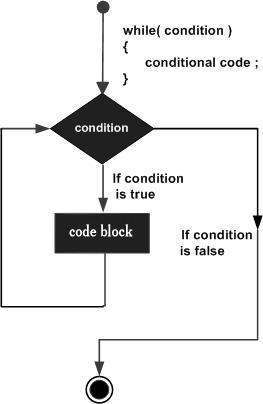
\includegraphics[width=0.4\linewidth]{../P2/img/whileloop.png}
		\caption{Flow chart perulangan while}
		\label{fig:whileloop}
\end{figure}

Syntaxnya pada bahasa C adalah sebagai berikut:
% Its syntax in C programming language is as follows
\begin{verbatim}
    while(Condition)
    {
        // Blok kode yang akan diulang
    }
\end{verbatim}

Sebagai contoh, perhatikan kode berikut
% As an example, look at the following code
\begin{lstlisting}[language=c,caption = Contoh Penggunaan while,label=lst:whileexample01]
int main()
{
	int uangSaya,hargaRoti;
	uangSaya = 10000;
	hargaRoti = 2000;
	while(uangSaya >= hargaRoti)
	{
	    printf("Beli roti 1, uang saya sisa %d", uangSaya - hargaRoti);
	    uangSaya -= hargaRoti;
	}
	printf("Uang saya tidak cukup lagi");
	return 0;
}
\end{lstlisting}  
Keluaran program di Listing \ref{lst:whileexample01} adalah sebagai berikut
\begin{verbatim}
    Beli roti 1, uang saya sisa 8000
    Beli roti 1, uang saya sisa 6000
    Beli roti 1, uang saya sisa 4000
    Beli roti 1, uang saya sisa 2000
    Beli roti 1, uang saya sisa 0
    Uang saya tidak cukup lagi
\end{verbatim}

Pada contoh ini, operasi pada baris 9 membuat variabel \verb|uangSaya| berkurang 2000 pada setiap pengulangan hingga akhirnya nilai \verb|uangSaya| tidak lebih dari atau sama dengan \verb|hargaRoti| lagi.
% You can see the line 9 of the code causes the variable \verb|uangSaya| to have its value substracted by 2000 for every loop until \verb|uangSaya| is no longer greater than equal to \verb|hargaRoti|. 
% The loop condition will be invalid and finaly exits the loop. Then it prints "Uang saya tidak cukup lagi", the command after the while loop statement.
Kondisi perulangan akan menjadi tidak valid dan akhirnya keluar dari perulangan. Kemudian ia mencetak "Uang saya tidak cukup lagi", perintah setelah pernyataan while loop.
\subsection{do-while loop}
do-while loop sebenarnya sama seperti while loop hanya saja do-while akan menjalankan perintah pada blok kode didalamnya terlebih dahulu sebelum melakukan pengecekan kondisi.
% do-while loop is very similar to while loop. The only difference is that do-while loop will execute the code block inside it once, and then checks the condition.
\begin{figure}[H]
		\centering
		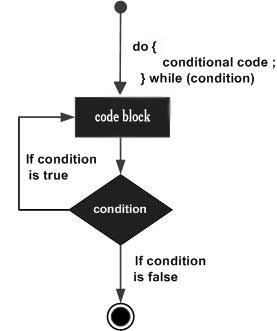
\includegraphics[width=0.4\linewidth]{../P2/img/dowhileloop.png}
		\caption{Pernyataan do-while}
		\label{fig:dowhileloop}
\end{figure}
Syntaxnya pada bahasa C adalah sebagai berikut:
% Its syntax in C is as follows:
\begin{verbatim}
    do{
        // the block of code that will be repeated
    }while(Condition)
\end{verbatim}
Sebagai contoh, perhatikan kode berikut
% Look at the following example.
\begin{lstlisting}[language=c,caption = Contoh Penggunaan do-while,label=lst:dowhileexample01]
int main()
{
	int uangSaya,hargaRoti;
	uangSaya = 10000;
	hargaRoti = 12000;
	do{
	    printf("Beli roti 1, uang saya sisa %d", uangSaya - hargaRoti);
	    uangSaya -= hargaRoti;
	}while(uangSaya >= hargaRoti)
	printf("Uang saya tidak cukup lagi");
	return 0;
}
\end{lstlisting}  
Output dari program pada Listing \ref{lst:dowhileexample01} adalah
% The output of the code above are
\begin{verbatim}
    Beli roti 1, uang saya sisa -2000
    Uang saya tidak cukup lagi
\end{verbatim}
% The variable \verb|uangSaya| is substracted by \verb|hargaRoti| before checking the \verb|uangSaya>=hargaRoti| condition.
% Had the code above uses while loop, the repeating block of code wouldn't have executed even once.
Variabel \verb|uangSaya| dikurangi dengan \verb|hargaRoti| sebelum memeriksa \verb|uangSaya>=hargaRoti| kondisi.
Seandainya kode di atas menggunakan perulangan while, blok kode yang berulang tidak akan dieksekusi sekali pun.
\subsection{Perulangan for}
Misalkan terdapat blok kode while dengan bentuk seperti ini:
% If you have a block of code like this:
\begin{verbatim}
    InitializationStatement; // e.g.: int i = 0;
    while(Condition){
        // do something
        updateStatement; // e.g.: i++ 
    }
\end{verbatim}
Hal ini setara dengan
\begin{verbatim}
    for(InitializationStatement;Condition;updateStatement){
        // do something
    }
\end{verbatim}

Sebagai contoh, perhatikan program berikut:
% As example, look at the following code:
\begin{lstlisting}[language=c,caption = Contoh Penggunaan for,label=lst:forexample01]
int main()
{
    int i=0;
    for(i=1;i<10;i++){
        printf("%d ",i);
    }
	return 0;
}
\end{lstlisting}
Output dari program ini adalah
% The output of this program are
\begin{verbatim}
    1 2 3 4 5 6 7 8 9 
\end{verbatim}
Berikut kode pada Listing \ref{lst:forexample01} jika diubah menjadi bentuk while-loop
% The following is the code if code in Listing \ref{lst:forexample01} converted to its while-loop form
\begin{lstlisting}[language=c,caption = For dalam bentuk while,label=lst:forwhileform01]
int main()
{
    int i=0;
    i=1;
    while(i<10){
        printf("%d ",i);
        i++;
    }
	return 0;
}
\end{lstlisting}

\section{Array}
Array atau biasa disebut larik adalah koleksi data dimana setiap elemen mempunyai nama yang sama dan bertipe sama. Setiap elemen diakses berdasarkan  indeks elemennya.
% Array is a collection of data where each element of it has the same name(indexed) and data type. Every element in an array can be accessed using its element index.
\subsection{Array 1D}
Variabel array dimensi satu dideklarasikan dengan menentukan jenis elemen dan jumlah elemen yang di perlukan oleh array. 
% One dimensional array variable can be declared by deciding the data type of the element and the number of element that is needed.

Syntax:
\begin{verbatim}
    DataType variableName [arraySize];
\end{verbatim}
\begin{enumerate}
	\item \verb*|DataType|.\\
    % The data type of the elements in the array, e.g. \verb|float|, \verb|int|, etc.
	Jenis elemen data elemen array :\verb*|float|,\verb*|int|,\verb*|char| dsb
	\item \verb*|variableName|\\
	Namariabel mengikuti aturan pemberian nama variabel,
    % variableName follows the variable naming convention
	
	\item \verb*|arraySize| \\
    % Integer more than 0. Defining the number of element an array has.
	konstanta integer lebih besar dari 0. \\
\end{enumerate}

Untuk menginisialisasi array dimensi satu, dapat dilakukan dengan cara seperti berikut:
% Initializing one dimensional array can be done like shown below:
\begin{verbatim}
    int contoh_array[5] = {4,2,0,6,9};
\end{verbatim}

Data di dalam array dapat akses dengan menggunakan suatu bilangan yang merupakan index dari array tersebut. Perhatikan potongan kode berikut.
% Data in an array can be accessed by using an integer that is the index of the array. Look at the code below

\begin{lstlisting}[language=c,caption = Contoh Mengakses Array 1D,label=lst:array1d01]
int main()
{
    int arr[5] = {4,2,0,6,9};
    printf("%d\n",arr[0]);
    printf("%d\n",arr[4]);
    int i = 0;
    printf("%d\n",arr[i]);
    for(i=0;i<5;i++)
        printf("%d",arr[i]);
}
\end{lstlisting}

Potongan kode pada Listing \ref{lst:array1d01} akan memberikan output
% The code in Listing \ref{lst:array1d01} will give output
\begin{verbatim}
    4
    9
    4
    42069
\end{verbatim}

\subsection{Array 2D dan Array Multidimensi lainnya}%Array 2D dan Array Multidimensi lainnya}
Array dimensi dua pada dasarnya hanya merupakan array dimensi satu dari array dimensi satu. Oleh karena itu, untuk mendeklarasikan array dimensi dua kita dapat menggunakan syntax seperti berikut.
% 2D array is basically a 1D array of 1D array. Intuitively, you can define a 2D array like as seen below:
\begin{verbatim}
	DataType variableName[arraySize1][arraySize2];
\end{verbatim}
Hal ini berlaku juga untuk array dengan dimensi lebih dari dua.
% This also applies to multidimensional array.
\begin{verbatim}
    DataType variableName[arraySize1]...[arraySizeN];
\end{verbatim}
Akan ada $arraySize_1\times arraySize_2 \times \cdots \times arraySize_n$ elemen yang akan dialokasikan ke memori setelah melakukan array multidimensi seperti itu
% There will be $arraySize_1\times arraySize_2 \times \cdots \times arraySize_n$ of elements that would be allocated to the memory after doing multidimensional array like that.

Untuk menginisialisasi suatu array multidimensi dapat dilakukan sama seperti array biasa:
% To initialize multidimensional array, you can do the following:
\begin{verbatim}
    int arr[2][2] = {{1,2},{3,4}};
\end{verbatim}

\subsection{Tugas Pendahuluan}
\begin{enumerate}
    \item Cobalah inisialisasi suatu array multidimensi dengan menggunakan perulangan for.
    % \item Try to initialize a multidimensional array with for loop
    \item Buatlah suatu program untuk mengisi data pada suatu array perdasarkan input dari keyboard.
    % \item create a program to fill the data of an array by keyboard input.
    \item Apakah yang akan terjadi jika suatu array \verb|arr| diakses dengan \verb|arr[-1]|?
    % \item What would happen if an array \verb|arr| is accessed with \verb|arr[-1]|?
    \item Apakah yang akan terjadi jika suatu array \verb|arr| dengan ukuran 5 diakses dengan \verb|arr[5]|?
    % \item What would happen if an array \verb|arr| with size 5 is accessed with \verb|arr[5]|?
    \item Lihatlah kode berikut
	% \item Look at the following code
    \begin{verbatim}
        for(i=0;i<10;i++){
            for(j=i;j<10;j++){
                printf("A");
            }
        }
    \end{verbatim}
    % How many "A" will be printed on the screen if that block of code is executed?
    Ada berapa banyakah huruf A yang akan muncul pada layar jika program tersebut dijalankan?
\end{enumerate}

\section{String}
Secara umum, string merupakan kumpulan dari satu atau lebih karakter. Spesifik pada bahasa C, string didefinisikan sebagai kumpulan karakter yang diakhiri oleh karakter null \verb|'\0'|.
\\
Misalkan string  \verb|"Dasar"|, pada bahasa C direpresentasikan sebagai kumpulan karakter \verb|'D'|, \verb|'a'|, \verb|'s'|, \verb|'a'|, \verb|'r'|, dan \verb|'\0'|.

\subsection{Penggunaan String}
Karena string tidak lain adalah array dari char, maka cara pembuatan tipe data string dalam bahasa C juga sama seperti cara pembuatan array. Berikut contohnya:
\begin{lstlisting}[language=c,caption = Contoh String dari Char,label=lst:array1d01]
	#include <stdio.h>
 
	int main(void)
	{
	char foo[8] = {'b','e','l','a','j','a','r','\0'};
	printf("Isi variabel foo adalah %s \n", foo);
	
	return 0;
	}
\end{lstlisting}

\verb|‘\0’| adalah salah satu syarat pembuatan string di dalam bahasa C. 
Semua string harus memiliki karakter “khusus” untuk menandakan akhir dari string. 
Tanda \verb|‘\0’| mewakili karakter null yang dipakai oleh compiler bahasa C sebagai tanda akhir sebuah string.

Contoh source code penggunaan \verb|scanf| untuk membaca string:
\begin{lstlisting}[language=c,caption = Contoh String dengan scanf,label=lst:array1d01]
	#include <stdio.h>

	int main() {
		// Mendeklarasikan variabel untuk menyimpan input dari pengguna
		int age;
		float height;
		char name[50];

		// Meminta pengguna untuk memasukkan usia mereka
		printf("Masukkan usia Anda: ");
		scanf("%d", &age);
		
		// Meminta pengguna untuk memasukkan tinggi mereka
		printf("Masukkan tinggi Anda (dalam meter): ");
		scanf("%f", &height);
		
		// Meminta pengguna untuk memasukkan nama mereka
		printf("Masukkan nama Anda: ");
		scanf("%s", name);

		// Menampilkan informasi yang dimasukkan pengguna
		printf("Nama: %s\n", name);
		printf("Usia: %d tahun\n", age);
		printf("Tinggi: %.2f meter\n", height);

		return 0;
	}
\end{lstlisting}

Contoh source code penggunaan 

\chapter{Fungsi (Subprogram)}
\section{Tujuan}
\begin{itemize}
    \item Students understand how to create and call functions in C %Mahasiswa mengerti cara membuat dan memanggil fungsi pada bahasa pemrograman C
    \item Students able to pass parameter by value and by reference in C.%Mahasiswa mampu menggunakan passing parameter by value dan by reference pada bahasa pemrograman C.
    \item Students understand and able to apply recursion in C. %Mahasiswa mampu mengerti dan mengaplikasikan konsep rekursi pada bahasa pemrograman C.
    
\end{itemize}   

The advantages of using functions in C programming language are:
\begin{itemize}
	\item Some code snippets can be reusable when using functions. 
\item We can call C functions any number of times in a program and from any place in a program.
\item Large C codes can be splitted to several function, thus easier to track.%Program c yang besar dapat dibagi ke dalam beberapa fungsi sehingga dapat dengan mudah untuk dilacak.
\end{itemize}
\section{Function Declaration}
 Every C program has atleast one function, that is the main() function. You can also define functions other than main().
 
Syntax :
\begin{verbatim}
    return_type function_name( parameters list){
        // function body
    	return something;
    }
\end{verbatim}
\begin{itemize}
	\item Return Type.\\ The data type a function has to return.
	\item \verb*|function_name|.\\ The name of the function
	\item parameters list.\\ %Nilai atau argumen yang menjadi input parameter. Urutan nilai yang dimaskuak ke fungsi berurutan sesuai dengan parameter yang dimasukan ke fungsi.
    The parameters of the function. 
	\item Badan fungsi.\\ The block of code that will be executed when the function is called.%Kumpulan statemen yang mendefinisikan apa yang dilakukan oleh fungsi.
	\item \verb|return something;|\\ A statement to return a value (\verb|something|). Returning the function causes the function to end.%merupakan statement untuk mengembalikan nilai dari fungsi. Untuk fungsi yang tidak mengembalikan nilai, dapat digunakan \verb|return_type| \verb|void|. Untuk keluar dari fungsi itu hanya perlu menggunakan statement \verb*|return|
    For functions that doesn't return a value (\verb|void| type function), ending the function can be done by using \verb|return;|
\end{itemize}
Example

\begin{lstlisting}[language=c]
float TriangleArea(float Base, float Height)
{
	float Area;
	Area = 0.5*Base*Height;
	return Area;
}
\end{lstlisting}


\section{Calling a Function} 

\begin{figure}[H]
	\centering
	\includegraphics[width=0.45\linewidth]{Fungsi/screenshot005}
	\caption{}
	\label{fig:memanggilfungsi}
\end{figure}

\begin{lstlisting}[language=c]
	#include <stdio.h>
// Mendeklarasikan fungsi luasSegitiga
// Parameter input ALas , dan Tintgi
// Output float
float TriangleArea(float Base, float Height)
{
	float Area;
	Area = 0.5*Base*Height;
	return Area;
}
int main()
{
	float Bs = 4,Hg=10,L;
    // Calling the TriangleArea function
	L=TriangleArea(Bs,Hg);
	printf("Area = %f",L);
	return 0;
}
\end{lstlisting}
\begin{enumerate}
	\item Line 5-10: Defining the function \verb|Triangle Area| with %Mendefunisikan fungsi \verb*|TriangleArea| dengan 
	\begin{itemize}
		\item Two input parameter :\\
	input \verb*|Base| and \verb*|Height|  with \verb*|float| data type.
	    \item Single valued output with \verb*|float| data type.
    \end{itemize}
\end{enumerate}
\section{Function with Arguments}
\subsection{Arguments}


%Jika suatu fungsi diharapkan untuk menggunakan argumen, maka variabel sebagai parameter yang menerima nilai dari argumen tersebut harus di dedeklarasikan terlebih dahulu. \\
\begin{enumerate}
	\item  \textbf{Parameter :}
\begin{enumerate}
	%\item Parameter adalah variabel dalam fungsi untuk merujuk ke salah satu bagian dari
	%data yang diberikan sebagai input ke fungsi.
    \item Parameters are the variable in the function that points to the part of the data that is inputted to the function.
	%\item Data ini disebut argumen.
    \item These data is called arguments.
	
\end{enumerate}

\item \textbf{Formal Parameter:}
\begin{enumerate}
	%\item Parameter yang Ditulis dalam Definisi Fungsi Disebut “Parameter Formal
    \item Parameter that is written within the function definition is called formal parameter.
    \item Formal Parameter is always a variable, Actual Parameter however doesn't necessarily has to be a variable.
	%\item Parameter formal selalu variabel, sedangkan parameter aktual tidak harus variabel.
	
\end{enumerate}


\item \textbf{Actual Parameter:}
\begin{enumerate}
	%\item Parameter yang Ditulis ketika memanggil fungsi
    \item Parameter that is used when calling the function
    \item Actual Parameter could take the form of number, expression, or another function call.
	%\item Dapat berupa angka, ekspresi, atau bahkan panggilan fungsi.
\end{enumerate}
\begin{figure}[H]
	\centering
	\includegraphics[width=0.7\linewidth]{Fungsi/screenshot006}
	\caption{}
	\label{fig:parameterformalaktual}
\end{figure}
\end{enumerate}
\subsection{Parameter Passing} 
%Passing parameter merupakan aktivitas menyalurkan nilai pada parameter saat memanggil fungsi. Pada umumnya, dikenal dua macam passing parameter yaitu:
To use a function with parameter, the parameters must be passed to the function first.
In general, there are two ways to pass paramater to a function
\begin{itemize}
	\item Pass parameter by value, pass the value of the variable to the function.%yaitu menyalurkan \textbf{nilai} dari tiap parameter yang diberikan.
	\item Pass parameter by reference, pass the reference of a variable (its memory address) to the function. %yaitu menyalurkan \textbf{alamat} dari tiap parameter yang diberikan.
\end{itemize}

\subsubsection{Passing Parameter by Value}

\begin{lstlisting}[language=c,caption = Passing by Value,label=lst:passbyvalue01]
#include<cstdio>
int swapAndReturnTheSum(int x, int y) {
    int z;
    z = x;
    x = y;
    y = z;
    return x+y;
}
int main()
{
    int a = 1;
    int b = 2;
    int sum = swapAndReturnTheSum(a,b);
    printf("sum: %d\n",sum);
    printf("values of a dan b now:\n");
    printf("a: %d\n",a);
    printf("b: %d\n",b);
}
\end{lstlisting}

%Perhatikan potongan kode pada Listing \ref{lst:passbyvalue01}. Baris 3-6 dari kode tersebut adalah operasi untuk menukar nilai dari 2 variabel. Namun, apabila program tersebut dijalankan, maka akan muncul output
line 3-6 of the code in Listing \ref{lst:passbyvalue01} is a set of assignments to swap the values of 2 variable. However, when the program is executed, the output would be the following.
\begin{verbatim}
    sum: 3
    values a and b now:
    a: 1
    b: 2
\end{verbatim}
The values of a and b did not swap. When passing parameter by value, anything that is done within the function body will have no effect on the parameter that is "passed on" the function. The value of the actual parameter will be assigned to the formal parameter, so we are not doing operation directly on the actual parameter.
%Nilai dari a dan b tidak bertukar. Untuk passing parameter by value, apapun yang dilakukan pada function body tidak akan berpengaruh pada parameter yang "dipassingkan". Nilai dari parameter aktual akan diassign pada parameter formal.

\subsubsection{Passing Parameter by Reference}
%Perhatikan baris 2 pada potongan kode berikut:
Look at line 2 of the following code.
\begin{lstlisting}[language=c,caption = Passing by Reference,label=lst:passbyreference01]
#include<cstdio>
int swapAndReturnTheSum(int &x, int &y) {
    int z;
    z = x;
    x = y;
    y = z;
    return x+y;
}
int main()
{
    int a = 1;
    int b = 2;
    int sum = swapAndReturnTheSum(a,b);
    printf("sum: %d\n",sum);
    printf("values of a dan b now:\n");
    printf("a: %d\n",a);
    printf("b: %d\n",b);
}
\end{lstlisting}
%apabila program tersebut dijalankan, maka akan muncul output
When this program is executed, it will output the following.
\begin{verbatim}
    sum: 3
    values of a and b now
    a: 2
    b: 1
\end{verbatim}

%Ketika fungsi \verb|swapAndReturnTheSum(a,b)| dipanggil, alamat memori variabel a dan b "dipassingkan" pada fungsinya. Sehingga pada pada potongan kode di baris 4-6, x dan y akan mengacu pada memori parameter aktual yang dimasukkan di baris ke 13. Ketika melakukan passing by reference, kita tidak bisa memanggil fungsi dengan parameter yang tidak memiliki alamat memori. Sebagai contoh \verb|tukarDanKembalikansumnya(1,2)| tidak bisa dilakukan karena angka 1 dan 2 bukan variabel dan tidak memiliki alamat memori.
When the function \verb|swapAndReturnTheSum(a,b)| is called, the memory address of \verb|a| and \verb|b| is passed on to the function. Therefore, in line 4-6, the \verb|x| and \verb|y| will point to the memory of the actual parameter that is inputted in line 13, so we are doing assignments directly to the actual parameter. When passing by reference, we can't call the function with parameter that has no memory address. As example \verb|swapAndReturnTheSum(1,2)| cannot be done as the number 1 and 2 doesn't have memory address.

\section{Recursion}
%Rekursi adalah ketika suatu fungsi dalam function bodynya memanggil fungsi itu sendiri.
%Sebagai contoh, perhatikan potongan kode berikut:
Recursion is when a function calls itself within its function body.
As an example, look at the code below.
\begin{lstlisting}[language=c,caption = Factorial with recursion,label=lst:recursionexample01]
int factorial(int n) {
    if (n==1)
        return 1;
    return n*factorial(n-1);
}
\end{lstlisting}
The factorial function calls another factorial function in line 4.
Initialy, the function $factorial(n)$ is called. This function however will return 
$n\times factorial(n-1)$, then $factorial(n-1)$ akan mengembalikan $(n-1)\times factorial(n-1-1)$.
Eventually it became like this:
%Dapat dilihat bahwa fungsi factorial pada function bodynya memanggil factorial pada baris 4.
%Pada awalnya jika fungsi $factorial(n)$ dipanggil maka dia akan mencoba untuk mengembalikan
\begin{equation*}
    \begin{split}
        factorial(n)& = n \times factorial(n-1)\\
        & = n \times (n-1) \times factorial(n-2)\\
        & = n \times (n-1) \times (n-2) \times \cdots \times 2 \times factorial(1)\\
        & = n \times (n-1) \times (n-2) \times \cdots \times 2 \times 1\\
    \end{split}
\end{equation*}

\section{Exercise}
\begin{itemize}
%    \item Buatlah fungsi yang dapat menerima 2 buah bilangan bulat a dan b kemudian mengembalikan nilai dari $a^b$
    \item Create a function that can take 2 integer a and b then returns $a^b$
%    \item Buatlah program dengan algoritma bubble sort tetapi proses penukaran 2 elemen pada array dilakukan dengan fungsi.
    \item Create program that do the bubble sort algorithm but the process of swapping 2 elements in the array is done with a function.
%    \item Masalah-masalah apa yang akan lebih mudah diselesaikan dengan menggunakan fungsi?
    \item What problems that can be solved easier with functions?
\end{itemize}

\end{document}